% !TEX root = ./thesis.tex
%\documentclass[phd]{pacotes/unb-cic}
\documentclass[bacharelado]{packages/unb-cic}%

%\usepackage[none]{hyphenat} %% diable hyphen
% \usepackage{fontspec} % MacOS
\usepackage[table]{xcolor}% http://ctan.org/pkg/xcolor
\usepackage[american,brazil]{babel}
\usepackage[T1]{fontenc}
\usepackage{indentfirst}
\usepackage{natbib}
\usepackage{xcolor,graphicx,url}
\usepackage[utf8]{inputenc}
\usepackage{booktabs} % for tables
\usepackage{verbatim} %% multiline comments
\usepackage{dirtytalk} %% Quotes
\usepackage{pdfpages}% incluir PDFs, usado no apêndice
\usepackage{multirow}
\usepackage{colortbl}
\usepackage{booktabs}
\usepackage{dirtree} 
\usepackage{changepage} 
\usepackage{subcaption}

\usepackage{epsfig}

\usepackage{listings}
\usepackage{packages/tikz-uml}

\newcommand\Tstrut{\rule{0pt}{3ex}}         % = `top' strut
\newcommand\Bstrut{\rule[-1.2ex]{0pt}{0pt}}   % = `bottom' strut

%% Algorithm
\usepackage[ruled,linesnumbered]{algorithm2e}
\usepackage{float}
\newfloat{algorithm}{t}{lop}
\floatname{algorithm}{Algorithm}
%% End Algorithm

%% definitions
\usepackage{amsmath}
\newtheorem{thm}{Theorem} % reset theorem numbering for each chapter
\newtheorem{defn}[thm]{Definition} % definition numbers are dependent on theorem numbers
%% end definitions

\graphicspath{ {imagens/} } % path to images



%% prof-reading
\usepackage[normalem]{ulem} % for \sout
\usepackage{xcolor}
\newcommand{\raw}{$\rightarrow$}
\newcommand{\ugh}[1]{\textcolor{red}{\uwave{#1}}} % please rephrase
\newcommand{\ins}[1]{\textcolor{blue}{\uline{#1}}} % please insert
\newcommand{\del}[1]{\textcolor{red}{\sout{#1}}} % please delete
\newcommand{\chg}[2]{\textcolor{red}{\sout{#1}}{\raw}\textcolor{blue}{\uline{#2}}} % please change
\newcommand{\issue[1]}{\marginpar{Issue\\#1}}

% Put edit comments in a really ugly standout display
\usepackage{ifthen}
\usepackage{amssymb}
\usepackage{amsfonts}
\newboolean{showcomments}
\setboolean{showcomments}{true} % toggle to show or hide \chapter{?}
\ifthenelse{\boolean{showcomments}}
  {\newcommand{\nb}[2]{
    \noindent\fcolorbox{gray}{yellow}{\bfseries\sffamily\scriptsize#1}
    {\sf\small$\blacktriangleright$\textit{#2}$\blacktriangleleft$}
   }
   \newcommand{\version}{\emph{\scriptsize$-$working$-$}}
  }
  {\newcommand{\nb}[2]{}
   \newcommand{\version}{}
  }

\newcommand{\gaa}[1]{\nb{Gabriel Ara\'ujo}{\footnotesize #1}}
\newcommand{\gab}[1]{\nb{Gabriel}{\footnotesize #1}}
\newcommand{\gena}[1]{\nb{Gena\'ina}{\footnotesize #1}}
\newcommand{\gio}[1]{\nb{Giovanni}{\footnotesize #1}}
\newcommand{\cris}[1]{\nb{Cristiane}{\footnotesize #1}}
%% end:prof-reading




%\bibpunct[; ]{(}{)}{,}{a}{}{;}%muda colchetes para parenteses

% definicoes previas do documento
%\selectlanguage{brazil}
\orientador[a]{\prof[a] \dr[a] Genaina Nunes Rodrigues}{CIC/UnB}
\diamesano{1}{December}{2020}
\author{Cristiane Naves Cardoso}
\title{Usando BDD para Testar Especificação de Missão em Ambiente de Robótica}
\palavraschave{dependabilidade}


\coordenador[a]{\prof[a] \dr[a] Célia Ghedini Ralha}{CIC/UnB}



\membrobanca{\prof[a] \dr[a]  Célia Ghedini Ralha}{CIC/UnB}
\membrobanca{\prof \dr Raian Ali}{Bournemouth University}


\CDU{004.4}

\palavraschave{dependabilidade}
\keywords{dynamic deployment, heterogeneous computing environment, context- and goal-oriented requirements engineering}

%-------------------------------------------------

\begin{document}

\maketitle

\pretextual
%\begin{agradecimentos}
%Agradecemos à nossa orientadora, \prof[a] \dr[a] Genaina Nunes Rodrigues,
%\end{agradecimentos}

%\begin{resumo}
%Nesse trabalho apresentamos...
%\end{resumo}

\selectlanguage{american}

\begin{abstract}%\textbf{}

% \input{parts/abstract}

\end{abstract}

\selectlanguage{brazil}
\tableofcontents
\listoffigures
\listoftables

\textual

\chapter{Introdução}
\label{chap:introduction}
Sistemas Multi-Robôs (SMR) são sistemas que consistem em mais de um agente robótico. Por algumas décadas esses sistemas foram utilizados em diversos contextos para cumprir diversas tarefas, especialmente em ambientes dinâmicos. SMRs atuam em um espaço ciber físico (i.e. parte do “mundo real”), logo seus agentes estão propensos à mudanças provenientes tanto de outros agentes do sistema como do ambiente em que estão inseridos \cite{iocchi2000reactivity}. Para aumentar a adaptabilidade do SMR, pode-se projetá-lo como um sistema auto-adaptativo, tornando-o capaz de responder à mudanças no ambiente, de maneira a continuar cumprindo objetivos e respeitando os limites impostos ao sistema \cite{sykes2010autonomous}.

Os agentes desses sistemas (i.e. robôs) existem no mundo físico e interagem com ele e entre si de maneiras mais complexas do que agentes de outros sistemas (e.g. computadores, bancos de dados, etc) \cite{cao1997cooperative}. Isso traz desafios para o desenvolvimento desse tipo de sistema, principalmente a preparação de experimentos com vários robôs \cite{noori20173d}. Essa dificuldade pode ser superada com o uso de simuladores.

Simuladores podem ser empregados tanto para testar a segurança, eficiência e robustez do sistema, quanto para prototipação de SMRs e robôs \cite{noori20173d}, \cite{pinciroli2012argos}. Outras vantagens de simuladores incluem: 

\begin{itemize}
    \item Menor custo de tempo e recursos para preparação e execução do experimento
    \item Ambientes simulados podem ser mais ricos, complexos e seguros que ambientes reais ou em laboratório \cite{robotSimulation}
    \item é possível testar hardware que não está disponível \cite{pinciroli2012argos},  \cite{echeverria2011morse}, \cite{robotSimulation}
\end{itemize}

De acordo com o Survey realizado \cite{robotSimulation}, muitos desenvolvedores de sistemas robóticos confirmam que simulações são ferramentas populares entre eles e um dos casos de uso mais comuns são os testes.

Diversos simuladores para SMRs existem na literatura, por exemplo Gazebo \cite{koenig2004gazebo}, Simbad \cite{hugues2006simbad}, CoppeliaSim \cite{rohmer2013coopeliasim}, MORSE \cite{echeverria2011morse} e Dragonfly \cite{maia2019dragonfly}, entre outros. Cada um desses simuladores foi criado com propostas diferentes, desde simulação precisa das partes que compõem um robô e sua interação com o ambiente (Gazebo, CoppeliaSim, Morse), até simulações de mais alto nível focando principalmente no comportamento dos robôs (Simbad, Dragonfly). Simulações multi-robô são suportadas por simuladores atuais, mas geralmente em menor número - devido ao alto uso de recursos computacionais necessários para simular cada robô (i. e. experimentos feitos com Gazebo mostraram que o simulador tem dificuldades ao simular mais de 10 robôs \cite{noori20173d}) - ou são muito específicos quando conseguem simular mais robôs (i.e. Dragonfly supostamente é capaz de simular até 400 entidades, mas está restrito à simulação de drones \cite{maia2019dragonfly}).

Ainda que simulações tenham um bom potencial, testes de campo são mais utilizados para validação e para verificação em sistemas robóticos do que os testes baseados em simulações. Alguns problemas dificultam o uso de simulações para fazer a validação e verificação (V\&V), dentre eles \cite{robotSimulation}:
\begin{itemize}
    \item Não ser possível ou dar muito trabalho para testar a aplicação com a GUI desabilitada;
    \item Não ser possível ou dar muito trabalho para executar a simulação sem intervenção manual;
    \item Não ter uma terminação clara da simulação (fechar a simulação no final da execução e mostrar os erros caso tenha algum);
    \item Interfaces instáveis;
    \item Dificuldades ao tentar reproduzir um resultado.
\end{itemize}

Mesmo com os diversos desafios, o autor \cite{robotSimulation} conclui que os desenvolvedores estão usando simulações para testar os seus robôs e muitos querem incorporar a simulação na rotina de automação de testes, mas é também sugerido fazer algumas mudanças:
\begin{itemize}
    \item Prover suporte para simulações sem a parte gráfica (GUI);
    \item Suporte para APIS estáveis e que tenham um bom design;
    \item Ter uma forma de reproduzir os resultados;
    \item Reduzir os custos de hardware (no caso de simulações pesadas).
\end{itemize}

O Laboratório de Engenharia de Software (LES) da Universidade de Brasília (UnB) conduz pesquisas na área de sistemas multi-agentes, incluindo sistemas multi-robôs. Entre os simuladores empregados nas pesquisas do LES, encontram-se Gazebo e MORSE, porém tem sido relatadas dificuldades com o uso desses simuladores em cenários com times maiores de robôs. Isso se dá pelo alto nível de detalhamento físico das simulações, que exige recursos computacionais consideráveis. Quando o objetivo da pesquisa é mais voltado para os algoritmos que coordenam os diferentes agentes do sistema, esse nível alto de detalhamento é desnecessário, mas aumenta consideravelmente o tempo de cada experimento.

Nesse cenário, parte da proposta deste projeto é fornecer uma ferramenta direcionada para simulação de sistemas multi-robôs auto-adaptativo com baixo nível de detalhamento físico. Esta ferramenta será usada na avaliação e comparar algoritmos de distribuição de tarefas entre agentes de um SMR. Também pode ser usado para prototipação das características de cada agente do SMR, bem como validação de requisitos do time de robôs de algum sistema.

Outra proposta deste projeto é como testar de forma automatizada as missões de uma simulação robótica, levando em consideração as dificuldades citadas anteriormente. Com este fim, será utilizado o Behavior Driven Development (BDD) para fazer a verificação e a validação dos comportamentos das missões.

\gio{Acho que a descrição do BDD tinha que ficar só no caítulo 2. Apresentar ele, como no parágrafo de cima parece o bastante. E eu diria também usar verbos no futuro (e.g. será usado) poderia ser trocada pro passado mesmo, porque a gente já fez o trabalho.}

Uma das ideias do BDD é validar o comportamento de uma determinada parte do software utilizando uma linguagem que pode ser entendida por todas as partes interessadas \cite{bddInAction}. O BDD será usado para criar diversos cenários de missões de simulação e verificar o comportamento da execução destes cenários.  Os cenários são compostos de várias regras e cada regra pode ser mapeada a um método que vai verificar se ela é executada corretamente. Para a criação dos cenários é utilizada linguagens que podem ser entendidas por todos os stakeholders, um exemplo é a linguagem Gherkin.


\gio{Melhor passar essa descrição de ECS pro capítulo 2, pra não ficar repetido}

Nesse padrão existem três elementos principais: as entidades, os componentes e os sistemas \cite{ecs_mmog_development}. As entidades representam um objeto único da simulação e é composta na maioria das vezes por apenas um identificador. Os outros dados relacionados à Entidade ficam guardados em outra estrutura, conhecida como Componente. 

O Componente é um container de dados que representa um aspecto do objeto, por exemplo, um componente de posição ou de renderização. Os Componentes possuem apenas dados, eles não possuem nenhuma lógica, nenhuma função para processar esses dados. Os responsáveis pela parte lógica são os Sistemas. 

Cada sistema será responsável por prover uma lógica, por exemplo, um Sistema de Renderização vai mostrar uma imagem na tela e um Sistema de Movimentação vai mover um objeto de um lugar para outro. Para realizar todos os processamentos, cada sistema receberá todos os componentes necessários para o seu funcionamento.  

Além do objetivo principal deste projeto, que é verificar a compatibilidade do BDD para testar de forma automatizada missões em um ambiente de robótica controlado, também será verificado se a arquitetura proposta facilitou o desenvolvimento dos testes e a criação dos cenários ou se trouxe alguma dificuldade adicional.

\section{Objetivos}

\gab{reformular os objetivos de forma a englobar outros aspectos do simulador que não só BDD}

O objetivo principal deste trabalho é analisar a compatibilidade do BDD com verificações de missões em ambiente de robótica.
\subsubsection{Objetivos Específicos}


Para analisar a compatibilidade do BDD com verificações de missões em ambiente de robótica, foram estabelecidos objetivos específicos:

\begin{itemize}
    \item Implementação da infraestrutura de simulação para o cenários (mapas, robôs, ações);
    \item Construir uma API para auxiliar nos testes das especificações das missões;
    \item Avaliar o desempenho do uso do BDD em ambiente de simulação de robótica.
\end{itemize}

\chapter{Referencial Teórico}
\label{chap:background}
% REFERENCIAL TEÓRICO
% ------------------- 
% Levantamento da literatura,
% conceitos importantes, 
% trabalhos relacionados
\label{chapter:referencial}

===> Completar falando da seção que discute herança vs composição

===> Completar dizendo que fala também do BDD


O referencial teórico apresenta conceitos importantes para o projeto e trabalhos relacionados encontrados na literatura. A Seção \ref{sec:outros_simuladores} descreve um breve levantamento feito de alguns simuladores bem estabelecidos na literatura. Esses projetos foram usados de inspiração para a criação do HMR Sim. A Seção \ref{sec:ECS} apresenta a \textit{design pattern} ECS (\textit{Entity-Compoenent-System}), analisada por ser bastante utilizada na criação de jogos, pela complexidade dos jogos de videogame atuais e como estes são de certa forma simuladores. Esta arquitetura foi utilizada no projeto do HMR Sim pelas suas vantagens. Finalmente a Seção \ref{sec:simulation_techniques} comenta sobre duas técnicas de simulação encontradas nos simuladores que foram levantados e na literatura.

\section{Simuladores na Literatura}
\label{sec:outros_simuladores}

O levantamento da literatura iniciou com um breve levantamento de simuladores já estabelecidos para sistemas robóticos. Foram selecionados os simuladores Gazebo \cite{koenig2004gazebo}, Simbad \cite{hugues2006simbad}, CoppeliaSim \cite{rohmer2013coopeliasim}, MORSE \cite{echeverria2011morse} e Dragonfly \cite{maia2019dragonfly}. Uma descrição breve de como os robôs são definidos em cada simulador é incluída, junto com um link para a documentação oficial do projeto.

\textbf{Gazebo.} Robôs são definidos em modelos, que seguem uma estrutura de arquivos definida. O robô em si é descrito em arquivos .sdf. Cada modelo é definido através de uma série de <links> que definem as partes do modelo. Sensores ou outros componentes - outros modelos - podem ser ligados através de <joints>. Modelos podem ter plug-ins com funcionalidade extra. O projeto é open source e pode acessado no link \url{http://gazebosim.org}. 

\textbf{CoppeliaSim.} Modelos são definidos como uma seleção de scene objects (e.g. joints, shapes, sensors, cameras, paths, etc). Existem muitas maneiras de controlar uma simulação, dentre elas destaca-se embedded scripts. Esse scripts podem ser definidos como parte de um scene object e executam alguma funcionalidade relacionada à este objeto. CoppeliaSim (antigamente V-Rep) é uma solução comercial da empresa Coppelia Robotics, disponível no link \url{https://www.coppeliarobotics.com/features}.

\textbf{MORSE.} Robôs são plataformas que definem o formato e certas propriedades, como área de colisão massa, etc. É nessas plataformas que sensores e atuadores são montados. Estes são fornecidos pelo simulador MORSE para serem adicionados à robôs. Apenas sensores e atuadores interagem com o mundo real com alguma funcionalidade. Os sensores e atuadores são fornecidos em diversos níveis de realismo, permitindo maior ou menor grau de abstração na simulação. MORSE é uma solução open source, baseado no software de modelagem Blender. Infelizmente o projeto se encontra abandonado desde 2020, mas ainda está disponível no link \url{https://morse-simulator.github.io}.

\textbf{Simbad.} Robôs são definidos em classes Java que estendem a classe \texttt{Agent}. Sensores são adicionados como atributos da classe. Status e movimentação do robô é alcançado através de APIs próprias. Robôs implementam as funções \texttt{initBehavior()} e \texttt{performBehavior()}, que definem o que acontece com o robô ao ser criado e o comportamento dele em cada loop de simulação. Um projeto open source disponível no link \url{http://simbad.sourceforge.net}.

\textbf{Dragonfly.} Drones possuem uma classe de controle - \texttt{DroneKeyboardController} ou \texttt{DroneAutomaticController}, respectivamente para ser controlado pelo usuário ou automaticamente. E classes que definem seus comportamentos, através de modelos. Além disso outras configurações, como nível de bateria, consumo por bloco, alvo e os wrappers (para fornecer comportamento adaptativo)  podem ser alterados pela interface gráfica, para cada drone na cena. Esse simulador está limitado à simuações de drones. Também open source, disponível em \url{https://github.com/DragonflyDrone/Dragonfly}.

Cada simulador possui características arquiteturais e objetivos próprios que foram analisados e comparados, fornecendo um arcabouço de técnicas que podem ser utilizadas (ver Tabela \ref{table:simulators_comparison}). Pontos relevantes que foram investigados sobre os simuladores incluem: 

\begin{itemize}
    \item \textbf{Nível de Abstração.} Pode ser \emph{baixo} indicando grande detalhamento dos componentes que compõe o robô e suas características físicas; \emph{médio} indicando necessidade de detalhamento dos movimentos individuais dos componentes que formam um robô; \emph{alto} indicando abstração dos componentes do robô.
    \item \textbf{Número de robôs} que o simulador é capaz de simular num tempo razoável
    \item Se o simulador é \textbf{genérico} ou não, ou seja, se existe restrição no tipo de robôs que o simulador é capaz de simular.
    \item \textbf{Arquitetura} utilizada na representação do robô (i.e. um robô é uma classe que deve ser implementada, ou um arquivo XML, etc). \emph{Declarativa} se refere à utilização de arquivos que representam um robo ou suas partes (e.g. descrição em arquivo XML); \emph{OOP} se refere à Programação Orientada a Objetos; \emph{MVC} indica o padrão \textit{Model View Controller}; \emph{AOP} faz referência à Programação Orientada a Aspectos.
    \item \textbf{Tipo de simulação} indica qual a técnica de simulação usada, em passos ou de eventos discretos (ver Seção \ref{sec:simulation_techniques})
\end{itemize}

\begin{table}[]
    \hspace{-0.8cm}
    \begin{tabular}{rccccc}
    \toprule

    \multirow{2}{25mm}{\textbf{Simulador}}      &
    \textbf{Nível de}                           &
    \multirow{2}{25mm}{\textbf{Nº de robôs}}    &
    \multirow{2}{25mm}{\textbf{Genérico}}       &
    \multirow{2}{25mm}{\textbf{Arquitetura}}    &
    \textbf{Tipo de}                            \\
    
                                    &
    \textbf{Abstração\Bstrut}       &
                                    &
                                    &
                                    &
    \textbf{Simulação\Bstrut}       \\

    \midrule

    {\textbf{Gazebo}\Tstrut} &
        {Baixo} &
        {\textless 20} &
        {SIM} &
        {Declarativa} &
        {Passos/DES} \\
        
    {\textbf{CoppeliaSim}\Tstrut} &
        {Baixo} &
        {\textless 20} &
        {SIM} &
        {Declarativa} &
        {Passos/DES} \\
        
    {\textbf{Simbad}\Tstrut} &
        {Médio} &
        {\textless 10} &
        {SIM} &
        {OOP} &
        {Passos} \\
        
    {\textbf{MORSE}\Tstrut} &
        {Médio/Alto} &
        {20 - 100} &
        {SIM} &
        {OOP/Declarativa} &
        {Passos} \\
        
    {\textbf{Dragonfly}\Tstrut} &
        {Alto} &
        {400} &
        {NÃO} &
        {MVC/AOP} &
        {Passos} \\
        
    \bottomrule
%     % {\textbf{HMR Sim*}} &
%     %     {\begin{tabular}[c]{@{}c@{}}Médio /\\ Alto\end{tabular}} &
%     %     {50 - 500} &
%     %     {SIM} &
%     %     {\begin{tabular}[c]{@{}c@{}}ECS/\\ Declarativa\end{tabular}} &
%     %     {\begin{tabular}[c]{@{}c@{}}Passos /\\ DES\end{tabular}}
    \end{tabular}
    \caption{Comparação resumida das ferramentas com suporte de simulação multi-robôs.}
    \label{table:simulators_comparison}
\end{table}


\section{Composição ao invés de herança}
\label{sec:heranca_composicao}

Como pode ser observado na Tabela \ref{table:simulators_comparison}, os simuladores observados utilizam em sua maioria métodos declarativos para definir os robôs, ou então Programação Orientada a Objetos (OOP, do inglês \textit{Object Oriented Programming}). OOP tradicionalmente utiliza \emph{herança} entre classes. O simulador criado nesse projeto, detalhado no capítulo \ref{chapter:hmr_sim}, utiliza uma combinação de métodos declarativos e \emph{composição}. Esta Seção discute brevemente a diferença entre herança e composição.

\subsection{Herança}
Herança permite o compartilhamento de dados e métodos entre classes de OOP, oferecendo uma solução para problemas de reuso e organização de código. Cada objeto no código é criado como uma instância de uma classe de forma que essa classe pode ou não herdar de outra classe. Quando uma classe filha/derivada herda de uma classe pai/base ela adquire todos os comportamentos do pai. A herança vai formar uma estrutura hierárquica em formato de árvore \cite{composition}, conforme mostra a figura \ref{fig:heranca}.

\begin{figure}
\centering
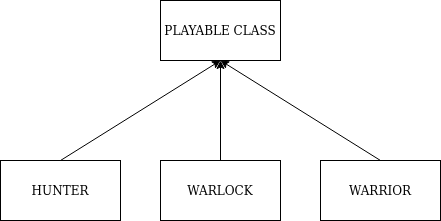
\includegraphics[scale=0.5]{imagens/heranca.png}
\caption{Herança Simples.} 
\label{fig:heranca}
\end{figure}

Uma hierarquia de classes utilizando Herança Simples é organizada como uma árvore, na qual cada nodo pode ter apenas um parente, ou seja, pode herdar de apenas uma classe. No caso, se uma entidade precisar herdar mais de um componente, este formato de árvore não é suficiente, sendo necessário o uso de Herança Múltipla. Neste tipo de herança, uma classe derivada pode extender de mais de uma classe pai.

Embora pareça uma solução fácil e simples no início, questões relacionadas ao uso de heranças múltiplas irão surgir. Um dessas questões é o problema do diamante, também conhecido como Deadly Diamond. Este é um problema de ambiguidade que ocorre quando duas ou mais classes, por exemplo, B e C herdam de uma classe A, e uma outra classe D herda de B e C, conforme a ilustração \ref{fig:deadlyDiamond}. Se existe um método em A no qual ambos B e C subscrevem e o método D não subscreve, então D vai herdar este método de B ou C?

\begin{figure}
\centering
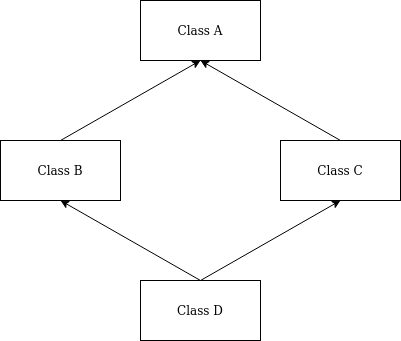
\includegraphics[scale=0.5]{imagens/deadly_diamond.png}
\caption{Deadly Diamond Problem.} 
\label{fig:deadlyDiamond}
\end{figure}

De acordo com Toni Härkönen, este tipo de Herança pode rapidamente se tornar trabalhosa para manter e expandir, uma vez que questões relacionadas a qual cópia da classe base será usada precisam ser resolvidas \cite{advantagesEcs}. Para resolver este problema, será necessário reorganizar a hierarquia de classes para se livrar do Deadly Diamond, provavelmente aumentando a repetição de código ou usando uma solução específica da linguagem de programação utilizada \cite{advantagesEcs}.

Outro problema no uso de Heranças é o acoplamento rígido da estrutura hierárquica de classes. Utilizando herança, um código com uma grande quantidade de entidades que herdam de outras entidades rapidamente vai possuir uma hierarquia de classes profunda. Alterar uma classe base, neste caso, pode causar efeitos colaterais indesejados em suas classes derivadas ou mesmo em todo o código \cite{composition}.

O problema citado anteriormente também é conhecido como \textit{Fragile base class}. Este é um problema de arquitetura da Programação Orientada a Objetos. Nele, as classes base são consideradas frágeis porque modificações aparentemente seguras na classe base, quando herdadas pelas classes derivadas podem causar um mal-funcionamento. Não dá para determinar se uma mudança é segura apenas examinando os métodos da classe base.

% falar sobre manutenibilidade

De acordo com Vittorio Romeo \cite{multiEcs}, considerando uma aplicação complexa ou um jogo que faz uso de uma arquitetura tradicionalmente orientada a objetos, as classes base são definidas como raízes de grandes hierarquias, das quais as entidades derivam. Com a adição de novos tipos de entidade, a complexidade do código aumenta, enquanto a capacidade de reutilização, flexibilidade e desempenho diminuem \cite{multiEcs}. 

Uma solução possível, segundo Toni Härkönen \cite{advantagesEcs}, é utilizar componentes ao invés de utilizar herança para agregar funcionalidades a um objeto. Resolvendo o problema do diamante e o problema do acoplamento rígido entre as classes.

Para Vittorio Romeo, uma abordagem alternativa mais poderosa consiste em usar um Design Orientado a Dados ou Composição, onde o código é projetado em torno dos dados e seu fluxo, e as entidades são definidas como um agregado de componentes \cite{multiEcs}.

O uso de Composição surge como uma alternativa ao uso de Herança.

\subsection{Composição}
A Composição permite a criação de tipos complexos combinando componentes de vários tipos, em vez de herdar de uma classe base ou pai \cite{composition}. Segundo Brian \cite{composition}, a composição contém instâncias de outras classes que implementam a funcionalidade desejada.

Fazendo uma analogia, é possível imaginar a Composição como um objeto montado de blocos de Lego. Várias peças de Lego (componentes) combinadas criam algo mais complexo, conforme mostra a figura \ref{fig:lego}. 

% como faço para citar uma imagem
\begin{figure}
\centering
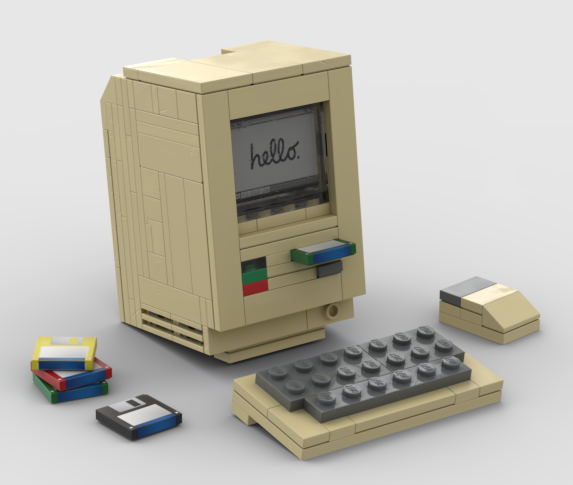
\includegraphics[scale=0.5]{imagens/macintosh.png}
\caption{Objeto construído combinando vários componentes.} 
\label{fig:lego}
\end{figure}

Este tipo de solução considera as mudanças futuras que podem ocorrer nos requisitos do software. Utilizando composição, não é necessário fazer uma reestruturação da árvore de classes, é possível simplesmente adicionar um novo componente à classe composta, sem modificar a superclasse para adaptar as mudanças \cite{composition}.

A figura \ref{fig:component} mostra como ficaria essa solução que utiliza um padrão conhecido como Object-Oriented Composition. Neste padrão, as entidades são compostas de pequenos componentes, que acrescentam funcionalidades a entidade. Estes componentes podem ser reutilizados em várias outras entidades. 

Um problema desta abordagem é que ela não dá suporte a separação dos dados e da lógica, ou seja, o componente possui os dados e a lógica na mesma estrutura. Uma outra abordagem proposta é utilizar um design que gerencia os dados de maneira mais eficaz, utilizando o padrão Entity Component System.

\begin{figure}
\centering
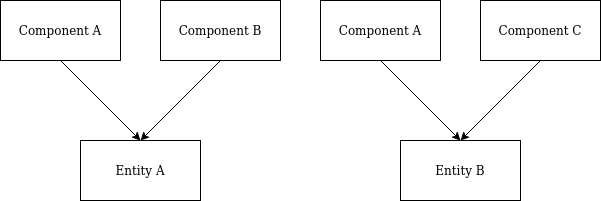
\includegraphics[scale=0.5]{imagens/component.png}
\caption{Object Oriented Composition.} 
\label{fig:component}
\end{figure}




\section{Entity-Component-System}
\label{sec:ECS}

O desenvolvimento de aplicações de tempo real e de jogos pedem por um sistema de gerenciamento de entidades que seja flexível e eficiente. \textit{Entity-Component-System} (ECS) é um padrão de desenho (\textit{design pattern}) de software amplamente utilizada em jogos, tipicamente em sistemas interativos em tempo-real (e.g. jogos do tipo MMO, \textit{Massive Multiplayer Online}) \cite{wiebusch2015decoupling}. 


Nesse padrão, objetos da simulação são transformados em \textit{entidades}. Uma entidade está relacionada a um conceito específico (e.g. uma parede, um robô, uma pessoa etc), com dados relacionados. Entidades podem ser criadas e destruídas ao longo da execução da simulação, e são usados apenas como identificadores. Cada entidade identifica uma coleção de \textit{componentes}. 

Um componente, por sua vez, armazena dados, mas tipicamente não implementa nenhuma lógica \cite{advantagesEcs}. Componentes também podem ser adicionados ou removidos durante a execução da simulação, alterando o estado da entidade à qual pertencem. Componentes representam algum atributo, estado ou capacidade da entidade (e.g. Posição, Velocidade, Sensores, etc). Dessa forma, o padrão ECS consegue separar dados da lógica da aplicação.

A lógica da simulação está nos \textit{sistemas}, que modificam os dados de componentes de acordo com seu objetivo \cite{multiEcs}. Em outras palavras, em vez de focar diretamente em uma entidade, os sistemas estão interessados em grupos de componentes que possuem os mesmos aspectos do sistema e que serão processados para realizar uma determinada tarefa \cite{advantagesEcs}. Cada sistema age de maneira independente de outros sistemas sobre um conjunto de componentes que lhe interessa. Ao mudar valores dos componentes, os sistemas efetivamente mudam o estado da simulação. O estado da simulação é o conjunto de estados de todos os componentes de todas as entidades presentes na simualção. Ele é alterado apenas pelos sistemas, cada um alterando uma pequena parte desse estado global. 

A figura \ref{fig:ecs} mostra o funcionamento de um sistema que usa o \textit{ECS}. Neste exemplo existem duas entidades: Robot e RechargeStation. A entidade Robot possui um componente Battery, Collidable, Velocity e Position e a entidade RechargeStation possui os componentes Station, Collidable e Position. As entidades serão discutidas na seção Entity e os componentes serão abordados na seção Components. 

\begin{figure}
    \centering
    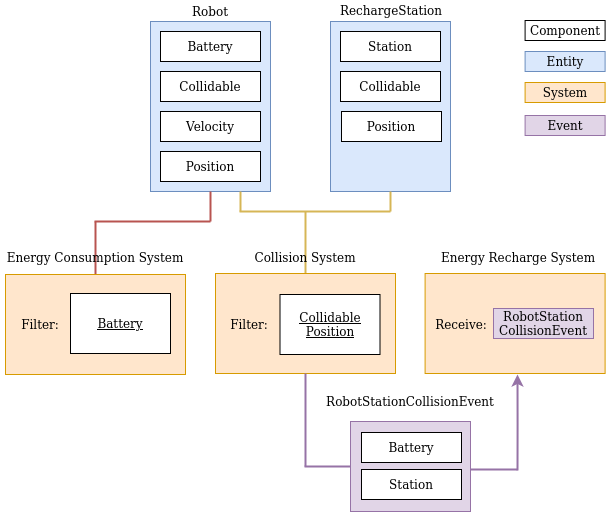
\includegraphics[width=\textwidth]{imagens/ecs.png}
    \caption{Exemplo de sistema construído no padrão ECS.} 
    \label{fig:ecs}
\end{figure}

O exemplo \ref{fig:ecs} apresenta dois sistemas. \texttt{Energy Consumption System} é responsável por consumir (decrementar) o total de energia de todas as entidades que possuem o componente \texttt{Battery}, sendo que nesse caso apenas a entidade Robot possui este componente. \texttt{Collision System} é responsável por verificar e notificar colisões entre entidades da simulação. Se ocorrer uma colisão entre uma entidade \texttt{Robot} e uma \texttt{RechargeStation}, significa que esse \texttt{Robot} quer recarregar a sua bateria. Sistemas são uma parte importante do simulador e são discutidos em maior detalhe na Seção \ref{sec:systems}.

% GIO: Achei muito detalhe isso aqui. Não creio que precisa ser incluído, mas não quis apagar. Talvez não concordem em remover
% e, portanto, o Collision System enviará uma notificação chamada RobotStationCollisionEvent para o sistema Energy Recharge System. O Energy Recharge System vai receber a notificação enviada e será responsável por recarregar a energia desse robô que está colidindo com a estação de recarga, incrementando o total de sua bateria. A parte de eventos, que é responsável por enviar notificações entre sistemas será melhor discutida na seção Eventos.

Essa organização permite grande modularização e separação de lógica entre as diferentes partes do sistema. Cada sistema (ou conjunto de sistemas) e seu conjunto de componentes associados pode ser adicionado ou removido do simulador conforme necessário, de maneira independente. Por exemplo, um sistema comunicação entre diferentes robôs pode ser implementado como um componente que guarde uma fila de mensagens e pode ser adicionado à cada robô, associado à dois sistemas: um sistema que faça a entrega das mensagens de um robô para o outro, e outro sistema que processa as mensagens de cada robô. Note que se o processamento não for adequado à uma simulação, basta trocar aquele sistema por outro que seja adequado. Além disso, se alguma simulação não faz uso desse sistema de mensagens, basta removê-lo do simulador completamente, deixando a simulação mais leve.

Uma outra vantagem de utilizar o padrão ECS é a flexibilidade de adicionar ou remover capacidades das entidades durante a execução da simulação. Como cada entidade é simplesmente uma coleção de componentes, é possível associar certas capacidades dos robôs (e.g. sensores, atuadores) à presença ou ausência de certos componentes naquela entidade. Por exemplo, dada a existência de um componente \texttt{camera} e um sistema associado que simule a captura de imagens, qualquer entidade que possue esse componente vai possuir a capacidade de coletar imagens via componente camera. Além disso, al simular falhas catastróficas em componentes, basta remover o componente da entidade sendo analisada.

Apesar dessas vantagens, como apontado por Wiebush \cite{wiebusch2015decoupling}, o uso de ECS pode trazer complicações de compatibilidade entre sistemas desenvolvidos de maneira indepentente, como uso de componentes incompatíveis, e dificuldade em conhecer qual sistema é responsável por determinada funcionalidade e como utilizá-la. detalhes de como esses problemas foram sentidos durante o desenvolvimento do projeto e medidas tomadas para mitigá-los são discutidas no capítulo \ref{chapter:hmr_sim}.

Foi utilizada a biblioteca \texttt{esper} para suporte do padrão ECS. Esper é uma biblioteca de ECS leve com foco em performance, escrita na linguagem Python por Benjamin Moran \cite{esper}. Ela cria uma classe \texttt{World} que mantém uma lista de entidades e de todos os componentes para cada entidade. Um componente pode ser qualquer estrutura em Python, no caso do projeto foram usadas classes (i.e. \texttt{class}). É possível ainda adicionar sistemas à classe \texttt{World}, que são implementados como funções, convencionalmente chamadas \texttt{process}. Alguns dos sistemas do projeto são adicionados ao \texttt{World}. \texttt{esper} também fornece funções que facilitam a obtenção de componentes ou conjuntos de componentes das entidades salvas, criação e remoção de entidades e componentes, e gerencia a execução dos sistemas.


\section{Técnicas de Simulação}
\label{sec:simulation_techniques}

Uma técnica de simulação bem estabelecida é a de tempo discreto com intervalo de incremento fixo \cite{belanger2010aboutsimulation}. Nesse modelo, o estado de um sistema no tempo $t_{i+1}$ é uma função do estado do sistema no tempo $t_i$. Cada variável que compõe o estado do sistema é uma função de variáveis e estados até o momento anterior. O incremento de tempo da simulação entre $t_i$ e $t_{i+1}$ é sempre o mesmo, e pré-definido.

Se o tempo $t_{calc}$ necessário para computar o estado $t_{i+1}$ do sistema a partir do estado $t_i$ é menor do que o tempo do incremento $t_{incr}$, então a simulação será computada mais rápido do que o tempo do relógio (e.g. o tempo real); da mesma forma, se $t_{calc} > t_{incr}$, então a simulação é computada mais devagar do que o tempo do relógio. Essas situações são conhecidas como simulação \textit{offline} \cite{belanger2010aboutsimulation}, porque não há sincronia entre o tempo da simulação e o tempo do relógio. Essa é uma situação aceitável para este projeto, onde o objetivo é obter a simulação desejada no menor tempo possível.

Essa técnica de simulação é indicada para simular sistemas que mudam constantemente, como por exemplo a temperatura de um ambiente ao longo do tempo, ou um sinal recebido por um sensor que trabalha a uma frequência conhecida. No entanto o  "relógio" da simulação é sincronizado, e todas as funções do estado são processadas a cada incremento de tempo, o que pode levar a cálculos desnecessários. Por exemplo, em uma simulação que involva uma função que altera temperatura de uma sala a cada 200ms, e um sensor que registra a temperatura da mesma sala com leituras a cada 100ms, a função que altera temperatura deve ser executada em todos os incrementos de tempo, que devem ser no máximo 100ms para suportar a leitura do sensor. Nesse cenário, metade das chamadas à função de alterar temperatura não afeta o estado do sistema, mas ainda tem que ser processadas.

Outra técnica de simulação é por eventos discretos (DES, \textit{Discrete Event Simulation}) \cite{matloff2008desintro}. Nesse modelo uma fila de eventos é processado um por vez, e cada estado $s_{i+1}$ é o resultado de processar o evento no topo da fila sobre o estado $s_i$. Um evento $e$ possui um tempo $t$ e uma função $f$ que altera o estado, e potencialmente cria outros eventos, que serão adicionados à fila. A fila de eventos é uma fila de prioridades ordenada pelo tempo $t$ de cada evento, sendo que o tempo de cada novo evento gerado pode ser igual ou maior que o tempo do evento que o gerou (nunca menor, porque não se pode alterar o passado da simulação). O tempo da simulação corresponde ao tempo $t$ do evento atual sendo processado, e como os eventos são ordenados pelo tempo, ele só será incrementado quando todos os eventos naquele tempo foram processados.

Diferentemente da simulação com intervalo de incremento fixo, onde as mesmas funções são executadas em intervalos conhecidos de tempo, na simulação do tipo DES funções diferentes alteram o estado da simulação, e o tempo da simulação no estado $s_i+1$ não depende apenas do estado $s$, mas também do evento sendo processado. Esse novo tempo pode não crescer de maneira uniforme ao longo da simulação. Essa técnica é adequada para simular sistemas que mudem de maneira infrequênte ao longo do tempo, por exemplo o inventário de um armazém \cite{belanger2010aboutsimulation}, ou a operação de robôs de serviço dentro do armazém. 

A simulação de incremento fixo de tempo pode ser implementada utilizando a técnica de eventos discretos, desde que os eventos sejam criados com tempos que possuam um intervalo constante. Uma outra característica interessante que pode ser alcançada com eventos discretos é separar a função em subsistemas que são executados de maneira independente e assíncrona. Retomando o exemplo da sala que muda de temperatura e possui o sensor, cada evento de leitura do sensor pode criar o próximo evento de leitura para o tempo $t + 100ms$; de forma similar cada evento de mudança de temperatura cria um novo evento de mudança para o tempo $t + 200ms$. Dessa forma, evita-se o problema de funções de alteração do estado da simulação tendo que ser executadas antes da hora.

O simulador utiliza a técnica de simulação de eventos discretos, através da biblioteca \texttt{simpy} \cite{simpy}. Esse framework de simulação DES é baseado em processos e faz todo o gerenciamento dos eventos e sua execução. A simulação acontece dentro de um ambiente, onde diversos processos interagem entre si e com o ambiente através de eventos. QUalquer função geradora em Python pode ser um process no simpy.

Esse framework também tem suporte para recursos (\textit{Resources}), que são compartilhados entre os processos. Recursos podem simular desde recursos a serem disputados (i.e. uma impressora, uma estação de carga) até recursos que são armazenados em contâiners (i.e. 10L de aguá de um reservatório com capacidade para 10000L). Recursos podem ainda ser preemptivos, ou filtrados de algum contâiner. Essa última capacidade foi bastante utilizada para a comunicação entre sistemas do simulador, como será discutido no Capítulo \ref{3_HMR_sim}.




%\subsection{Data-Oriented Design}
%No desenvolvimento de softwares computacionalmente mais pesados, um %problema frequente é o desempenho, que faz com que o tempo de execução %do programa para diferentes tarefas parem por tempos inaceitáveis %\cite{advantagesEcs}. Podem existir diferentes motivos para isso %ocorrer, como, por exemplo, algoritmos não otimizados, mas este não é o %principal caso. Para Toni Härkönen, é bastante comum que a lentidão %seja causada pelo gerenciamento ineficiente da memória. Uma solução %para este problema é utilizar um design que gerencia os dados de %maneira eficaz, portanto, o autor sugere uma mudança de pensamento %orientado a objetos para o design orientado a dados %\cite{advantagesEcs}.

% Falar sobre manutenibilidade e extensibilidade.

\subsection{Comunicação entre sistemas}
Um sistema muitas vezes terá a necessidade de se comunicar com outros sistemas. O uso de eventos dá suporte para estas comunicações.
\subsubsection{Eventos}
Uma parte importante das arquiteturas de softwares voltadas a jogos são os Eventos.
Eventos são ações que podem ser geradas quando um determinado comportamento ocorre em um determinado sistema, sendo enviados para um ou mais sistemas que terão como uma de suas atividades tratar a ocorrência dessas ações. Por exemplo, um evento de colisão, no qual duas entidades podem se colidir e quando isso ocorrer será enviado um evento para um Sistema responsável por tratar essa ocorrência.

Existem diferentes formas de tratar a ocorrência de eventos e muitas bibliotecas que lidam com \textit{Entity Component System} possuem um sistema de gerenciamento capaz de tratá-los. Também existem diferentes bibliotecas em várias linguagens para o tratamento de eventos (não apenas para jogos). Em python, por exemplo, existe a biblioteca PyDispatcher, que fornece um serviço centralizado para entrega de mensagens a objetos registrados \cite{pydispatcher} e também tem a biblioteca \textit{zope.event} \cite{Zope} que segue o padrão \textit{Observer}, entre várias outras bibliotecas.

Utilizando o padrão Observer é possível enviar a notificação da ocorrência de um evento para sistemas que ficam esperando a ocorrência desses eventos.

%Dependendo da forma como o tratamento de eventos ocorre, um determinado %sistema fica verificando a cada update todos os componentes %relacionados a ele para encontrar apenas as entidades necessárias para %realizar alguma lógica. Por exemplo: um sistema de Colisão vai procurar %todas as entidades que possuem um componente \textit{Collidable} e para %cada componente desse vai ter outra iteração por todos os componentes %\textit{Collidable} para verificar se ocorreu alguma colisão entre dois %componentes. 

%Dessa maneira o custo total de iterações para cada sistema acaba se %tornando maior conforme o número de sistemas e de entidades aumentam.

%Uma outra forma de lidar com eventos é utilizar padrões parecidos com o %\textit{Observer}, no qual não é necessário iterar toda vez sob todos %os objetos. Utilizando o padrão Observer é possível enviar a %notificação da ocorrência de um evento para sistemas que ficam %esperando a ocorrência desses eventos. 

\subsubsection{Observer Pattern}

\gio{Isso aqui é usado nos testes? Não vi muito sentido em explicar isso (do ponto de vista do simulador)}
O Padrão Observer é um Behavioral Pattern que define uma dependência entre objetos do tipo one-to-many de forma que quando um objeto muda o seu estado, todos os seus dependentes são notificados e atualizados de forma automática \cite{gamma1994design}.

O padrão \textit{Observer} permite definir um sistema de notificações no qual um objeto, conhecido como \textit{Subject}, pode enviar eventos para outros objetos, conhecidos como \textit{Observers}, que ficam esperando (observando) por essas notificações. Para isso, o \textit{Subject} mantém uma lista de dependentes do tipo \textit{Observers} e quando ocorre uma mudança no seu estado é enviado uma notificação para todos os \textit{Observers} dessa lista.

Este tipo de interação também é conhecida como Publish-Subscribe \cite{gamma1994design}. O Subject é o Publisher (publicador) das notificações e os Observers podem ser descritos como Subscribers.

Para diminuir o acoplamento e para que o \textit{Publisher} não precise saber da implementação de todos os \textit{Subscribers} é importante que se utilize uma mesma interface entre os \textit{Subscribers} e que o \textit{Publisher} possa se comunicar com eles através dessa interface \cite{observer}.

A estrutura do Observer Pattern é ilustrada pela figura \ref{fig:observer}. Este exemplo possui os seguintes participantes:
\begin{itemize}
    \item Subject:
        \begin{itemize}
            \item Guarda os estados de interesse dos Observers;
            \item Provê um meio de registrar e de cancelar o registro de um observer;
            \item Envia notificações para os observadores quando ocorre mudanças no estado;
            \item Guarda uma lista de Observers.
        \end{itemize}
    \item Observer:
        \begin{itemize}
            \item Define a interface para atualizar os objetos que serão notificados da mudança no Subject.
        \end{itemize}
    \item ConcreteObserver:
        \begin{itemize}
            \item Implementa a interface de update (atualização) do Observer.
        \end{itemize}
\end{itemize}

\begin{figure}
\centering
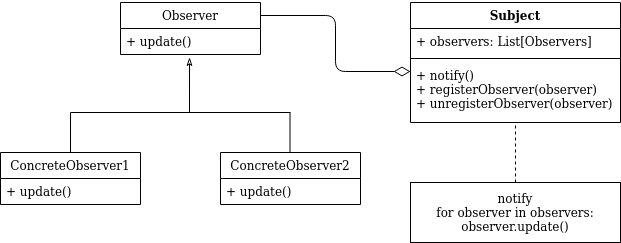
\includegraphics[width=\textwidth]{imagens/observer.png}
\caption{Observer Pattern.} 
\label{fig:observer}
\end{figure}

%TODO não se referencia Wikipédia em trabalho academico. A referência padrão em design patterns é o livro "Design Patterns: Elements of Reusable Object-Oriented Software - Erich Gamma, Richard Helm, Ralph Johnson, and John Vlissides, with a foreword by Grady Booch."

%Atualmente o projeto utiliza duas formas de tratamento de eventos: o %tratamento de eventos do gerenciador de ECSs Esper e o tratamento de %eventos do Simpy.

%O tratamento de eventos do Esper segue um padrão de comunicação entre %componentes. O sistema responsável por tratar um determinado tipo de %evento faz uma busca por todas as entidades que possuem certos tipos de %componentes. Por exemplo, um Sistema de Colisão precisa acessar todas %as entidades que possuem todos os três componentes: Collidable, %Position e Velocity.

% section simulacao
% subsection simulacao utilizando ECS

\section{Behavior Driven Development}
O BDD é um conjunto de práticas da Engenharia de Software que tem como propósito melhorar a qualidade do código e a entrega de um software correto \cite{bddInAction}. O BDD baseia-se em práticas Ágeis e do Lean, utilizando principalmente técnicas do DDD (Domain-Driven Design) e do TDD (Test-Driven Development).

O BDD propõe o uso de uma linguagem que é entendível por todos os stakeholders. Desta forma, todos os envolvidos vão utilizar essa linguagem para descrever as funcionalidades do software, que serão descritas em vários arquivos que terminam com o sufixo .feature. Uma das ideias do BDD é utilizar estes arquivos como uma forma de documentação e também para testar os vários comportamentos do software.

As features e os cenários dela descrevem os requisitos do software e serão usadas como casos de teste. Cada arquivo .feature será responsável por descrever um ou mais cenários.

Os cenários são compostos de várias regras e cada regra pode ser mapeada a um método que vai verificar se ela é executada corretamente. Para a criação dos cenários é utilizada linguagens que podem ser entendidas por todos os stakeholders, um exemplo é a linguagem Gherkin.

Uma feature pode ser especificada da seguinte forma \cite{BDDthesis}:

\textbf{Feature}: breve descrição da funcionalidade

\textbf{Background}: agrupa regras que são comuns em todos os cenários.

\textbf{Scenario}: descrição de um cenário específico da funcionalidade.

\hspace{1cm}\textbf{Given} uma pre-condição

\hspace{1cm}\textbf{And} outra pre-condição

\hspace{1cm}\textbf{When} ocorre uma ação

\hspace{1cm}\textbf{And} outra ação ocorre

\hspace{1cm}\textbf{Then} é obtido um resultado testável

Cada keyword do Gherkin\footnote{https://cucumber.io/docs/gherkin/reference/} descrita acima é responsável por:
\begin{itemize}
    \item \textbf{Feature}:
    O propósito da keyword feature é dar uma descrição de alto nível de uma funcionalidade do sistema e agrupar os cenários relacionados a esta feature.
    \item \textbf{Background}:
    Quando uma ou mais regras Given estão sendo repetidas em todos os cenários, elas podem ser agrupadas na seção do Background. As regras agrupadas nesta seção serão executadas antes dos cenários.
    \item \textbf{Scenario}:
    A keyword Scenario descreve uma regra de negócio da funcionalidade e é composto por várias regras Given/When/Then.
    \item \textbf{Scenario Outline}:
    Permite executar um cenário várias vezes e a cada vez utiliza exemplos de valores diferentes. Os valores serão definidos com a keyword Examples.
    \item \textbf{Examples}:
    Permite criar uma tabela de exemplos. Cada coluna da tabela representa uma variável e cada linha vai conter um valor diferente para a variável. Estes exemplos podem ser usados quando um cenário é executado várias vezes, dessa forma, a cada vez que um cenário é executado é lida uma linha da tabela de exemplos.
    \item \textbf{Steps}
    Descreve os passos necessários para completar um cenário. Estes passos podem ser dos seguintes tipos:
    \begin{itemize}
        \item \textbf{Given}:
        Define um estado inicial antes de começar a testar. Nesta etapa podem ser feitas instâncias de objetos, configurações de banco de dados, busca por uma página da web, entre outras configurações necessárias para deixar o sistema em um estado inicial.
        \item \textbf{When}:
        Define um evento ou uma ação que será realizada no sistema que está sendo testado. Esta ação pode ser feita por uma pessoa ou por um outro sistema. 
        \item \textbf{Then}:
        Descreve o resultado esperado da execução das etapas anteriores. Nesta etapa será realizado o assert para verificar se o output recebido é igual ao output que era esperado.
        \item \textbf{And/But}:
        Serve como um sinônimo para o passo anterior a ele e é utilizado para evitar várias escritas do Given/When/Then.
    \end{itemize}
    
    
\end{itemize}

\gab{TODO ao invés de image, usar listing com highlight para Gherkin
% ref: https://gist.github.com/nsommer/9a04f6ebc6ea8b9f5b816becb97e7d9b
}

\begin{figure}
\centering
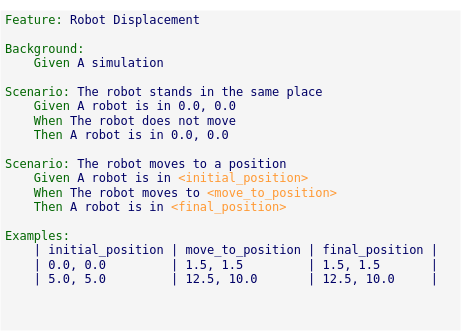
\includegraphics[width=\textwidth]{imagens/bddExample.png}
\caption{Exemplo de um arquivo .feature} 
\label{fig:bddExample}
\end{figure}

A figura \ref{fig:bddExample} mostra um exemplo de um arquivo .feature.

Um problema que o BDD tenta resolver é a comunicação entre os times e demais stakeholders e a perda de informações das features ao longo dos diversos processos. Por exemplo, utilizando o BDD, quando uma pessoa da área de negócios pede por uma nova feature, ela vai se reunir com o time de desenvolvedores e de testadores e vai explicar os requisitos dessa nova feature. Nesta reunião, todos os envolvidos vão traduzir essas especificações, utilizando a linguagem Gherkin, em cenários e regras que podem ser entendidos por todos os envolvidos. Os diversos cenários e regras descritos vão guiar o desenvolvimento da feature e vão servir como casos de teste \cite{bddInAction}.

De acordo com \cite{bddInAction}, o BDD vai ajudar o time a focar na identificação, no entendimento e na implementação das features que realmente importam para os clientes.


\section{Simulações Robóticas}

\gio{ Acho essa seção desnecessária. Tudo que tem aqui já foi falado na introdução. Melhor falar tudo lá, até porque faz parte do contexto do projeto.}

Simulações robóticas são ferramentas importantes para o processo de design, de prototipação, de desenvolvimento e da verificação e validação de um sistema robótico. Sendo uma opção mais viável e barata do que fazer testes em campo \cite{robotSimulation}. Essas simulações são usadas na maioria das vezes para fazer testes, podendo ser usadas para testar algoritmos, componentes, sistemas multi-robôs, dentre outros tipos de sistemas. O artigo \cite{robotSimulation} mostra que os desenvolvedores enxergam valor em utilizar simulações para testes e que esses desenvolvedores utilizam simulações quando é impraticável fazer os testes em um hardware ou outro ambiente real.


\subsection{Dificuldades}
Mesmo tendo um bom potencial, o uso de simulações possui vários desafios e dificuldades, conforme foi relatado por desenvolvedores da área da robótica \cite{robotSimulation}.

As principais dificuldades relatadas \cite{robotSimulation} ao usar simulações foram:

\begin{itemize}
    \item \textbf{Diferença entre realidade e simulação}: Existe uma grande discrepância entre a realidade e a simulação. Muitas vezes existe uma inadequação da representação da física no simulador ou a produção de comportamentos não realistas.
    \item \textbf{Complexidade}: É referente às dificuldades adicionais na usabilidade do simulador. Serão gastos tempo e recursos que poderiam ser gastos em outras atividades. Conforme relatado, sairia mais fácil e mais acurado configurar e testar em um sistema físico real.
    \item \textbf{Falta de funcionalidades}: Os simuladores não possuem todas as funcionalidades desejadas pelo desenvolvedor ou se possuem são bastante caros. Cada simulador é bom em um determinado aspecto, mas nenhum é bom em todos eles. 
    \item \textbf{Documentação}: Falta de documentação ou documentação errada.
\end{itemize}

Dificuldades relacionadas a construção de testes \cite{robotSimulation}:
\begin{itemize}
    \item \textbf{Reprodutibilidade}: É difícil repetir o resultado de uma simulação, pois ela é não determinística.
    \item \textbf{Construção de cenários e ambientes}: Os desenvolvedores relataram ter dificuldade ao criar os cenários para os testes.
\end{itemize}

Desafios que afetam a automação dos testes \cite{robotSimulation}:
\begin{itemize}
    \item Não ser possível rodar os testes sem desabilitar a GUI é uma das maiores dificuldades da automação dos testes.
    \item Rodar a simulação sem intervenção manual.
    \item Não ter uma terminação clara da simulação.
    \item Interfaces instáveis.
\end{itemize}


\chapter{O simulador HMR Sim}
% Label chapter:hmr_sim
\label{chapter:hmr_sim}

Conforme comentado no Capítulo \ref{chap:introduction}, a proposta deste projeto é fornecer uma ferramenta direcionada para simulação de sistemas multi-robôs auto-adaptativo com baixo nível de detalhamento físico. Essa porposta foi realizada através do simulador HMR Sim. É um projeto \textit{open source}, disponível em \url{https://github.com/lesunb/HMRSsim}.

A linguagem escolhida foi Python, uma linguagem de programação popular e versátil. Outros simuladores analisados têm suporte para essa linguagem, como MORSE e CoppeliaSim. Arquitetura do simulador é baseado na \textit{design pattern} Entity-Component-System (ECS), e a técnica de simulação é de eventos discretos. Grande foco foi dado para modularização e reaproveitamento de sistemas na construção do simulador. Alguns dos principais sistemas (e.g. Navegação, Script) foram construídos para serem extensíveis. Além disso foi dado atenção à facilidade e rapidez de construir simulações. A arquitetura do simulador é detalhada na Seção \ref{sec:architecture}. A criação e uso de sistemas na Seção \ref{sec:systems}. Os principais sistemas já construídos são apresentados na Seção \ref{sec:systems_available}, incluindo o sistema que permite visualização da simulação, Seer. Finalmente a Seção \ref{sec:performance} verifica o desempenho do simulador numa simulação com grande número de robôs.

Uma simulação no HMR Sim tem dois estágios: (1) fase de carregamento, onde os componentes disponíveis são carregados e as entidades da simulação criadas e (2) fase de execução, onde os sistemas da simulação são inicializados e a simulação em si é executada. Componentes são definidos como classes em Python e são carregados automaticamete utilizando um sistema de nomenclatura apropriado. Sistemas são construídos como funções Python, e podem ser processos da biblioteca \texttt{simpy} ou funções aceitas como sistemas do \texttt{esper} (ver Seções \ref{sec:simulation_techniques} e \ref{sec:ECS} para detalhes sobre as bibliotecas). Os sistemas devem ser inicializados e adicionados ao simulador antes da fase de execução. A Seção \ref{sec:ents_and_components} cobre a criação de componentes e como eles ficam disponíveis no simulador.

Uma simulação pode ser definida em um mapa (veja figura \ref{fig:example_map}), programaticamente através de um objeto de configuração (dicionário Python), ou uma mistura das duas opções. Mapas são arquivos XML construídos com a biblioteca \texttt{JGraph} (disponível em \url{https://github.com/jgraph}), com algumas restrições. Qualquer programa compatível com essa biblioteca pode ser utilizado, por exemplo \url{diagrams.net}, bastante popular. Também é possível criar entidades na simulação através de \textit{EntityDefinition}.

As formas desenhadas no mapa da simulação podem ser anotadas para especializá-las (marcar a figura como um certo tipo de entidade), adicionar componentes, ou diferenciá-la de alguma forma. Na figura \ref{fig:example_annotations}, por exemplo, as anotações marcam aquele objeto do mapa como um robo, que possui um componente \texttt{Claw} inicializado com os valores \texttt{[80, 1]}, e um componente \texttt{Script} inicializado com os valores da figura.

\begin{figure}[ht]
    \centering
    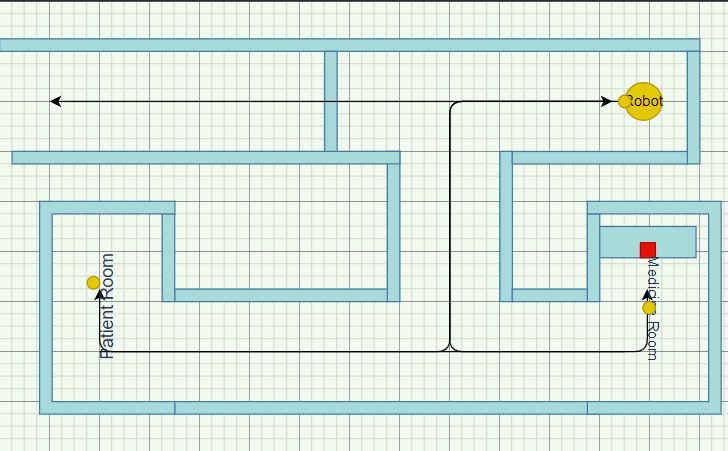
\includegraphics[width=.8\textwidth]{map_example.png}
    \caption{Exemplo de mapa de uma simulação}
    \label{fig:example_map}
\end{figure}

\begin{figure}[ht]
    \centering
    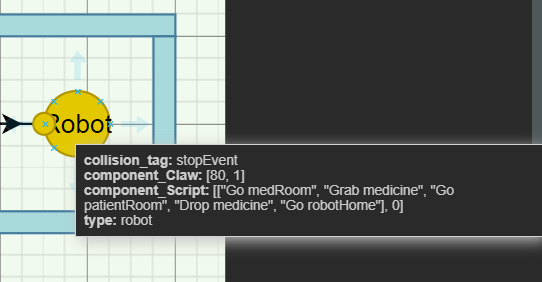
\includegraphics[width=.8\textwidth]{robot_annotations.png}
    \caption{Exemplo de anotações em uma entidade}
    \label{fig:example_annotations}
\end{figure}


\section{Arquitetura}
\label{sec:architecture}

\begin{figure}[ht]
    \centering
    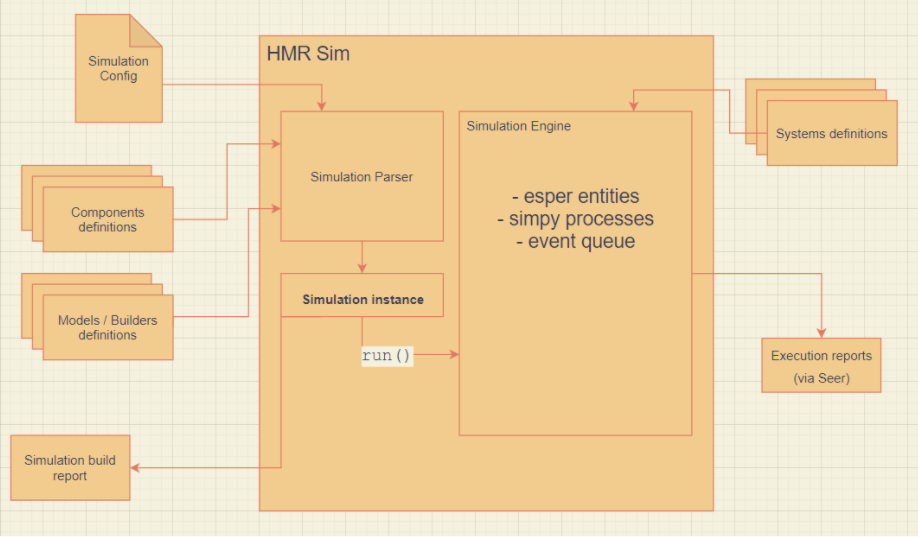
\includegraphics[width=\textwidth]{architecture_overview.png}
    \caption{Diagrama representando um resumo da arquitetura do HMR Sim}
    \label{fig:architecture_overview}
    \gab{reexportar imagem como pdf}
\end{figure}

A figura \ref{fig:architecture_overview} mostra um resumo da arquitetura do simulador HMR Sim. A construção da simulação acontece separada da simulação em si. Para construir uma simulação, um objeto de configuração tem que ser passado para o simulador, bem como as definições dos componentes disponíveis e os \texttt{models} e \texttt{builders} disponíveis. A classe \texttt{Simulator} cria a simulação, e depois a executa. A instancia da simulação mostrada na figura \ref{fig:architecture_overview} (\textit{Simulation instance}) é exatamente a instância da classe \texttt{Simulator} criada.

O objeto de configuração é um dicionário Python, que pode ser salvo como um arquivo \texttt{json}. Algumas das opções mais importantes estão listadas abaixo. Para ver todas as opções verifique a documentação do projeto, no repositório.

\begin{itemize}
    \item \textbf{context} (string) - A raíz do projeto, de onde componentes, sistemas e builders extras serão incluídos;
    \item \textbf{map} (string) - O arquivo XML do mapa
    \item \textbf{FPS} (int) - Frequência com que serão executados os sistemas do \texttt{esper}. Esses sistemas não geram eventos, são indicados para representar sistemas que acontecem de forma frequênte e previsível. Caso nenhum sistema \texttt{esper} seja utilizado não é necessário informar esse valor.
    \item \textbf{duration} (int) - Tempo limite da simulação (no relógio da simulação). Por exemplo, um valor 6 vai fazer o simulador encerrar a simulação após 6s serem simulados.
    \item \textbf{simulationComponents} (dict) - Componentes "globais". Eles são adicionados à entidade 1, reservada à simulação. Podem ser acessados por todos os robôs (e.g. um mapa compartilhado de rotas).
    \item \textbf{extraEntities} (EntityDefinition[]) - Lista de \texttt{EntityDefinition} (ver documentação), que definiem entidades que não estão presentes no mapa mas devem ser incluídas na simulação. É possível declarar todas as entidades com essa opção e usar o mapa apenas para coisas estáticas, reaproveitando-o para vários cenários. 
\end{itemize}

O simulador importa automaticamente \texttt{components}, \texttt{models} e \texttt{builders} do sistema de arquivos. Por conta disso os projetos que usem o HMR Sim precisam de uma organização expecífica, como mostrado abaixo. Dentro de cada pasta os arquivos deve estar no formato apropriado.

\begin{lstlisting}[]
                   project_root     
                    |                 
                    |-- models        
                    |-- components    
                    |-- builders      
\end{lstlisting}

A simulação construída se torna uma instância da classe \texttt{Simulator} cujo atributo \texttt{World} está preenchido com as entidades que foram criadas, e as opções de configuração salvas. Essa instância é um objeto Python, podendo ser salvo através da biblioteca \texttt{pickle}, por exemplo, e distribuído. Antes de poder ser executada, no entanto, é necessário inicializar e adicionar os sistemas à simulação. Para adicionar sistemas os métodos \texttt{Simulator.add\_system} e \texttt{Simulator.add\_des\_system} podem ser usados. Qual dos dois usar depende do sistema a ser adicionado, detalhes na Seção \ref{sec:systems}.

Após adicionar os sistemas, a simulação pode ser executada utilizando o método \texttt{Simulator.run}, da instância do simulador gerada. A simulação é executada por \texttt{duration} segundos de simulação, se essa opção foi passada na configuração, ou até que o evento \texttt{KILL\_SWITCH} seja processado. É possível manter ver logs da simulação durante a execução. A visualização gráfica da simulação é implementada através do sistema Seer, discutido na seção \ref{sec:seer}.

Alguns sistemas com funcionalidades consideradas essenciais na maior parte das simulações já foram implementados, como parte da validação do simulador. Eles serão detalhados na Seção \ref{sec:systems_available}, e incluem sistema de navegação, movimentação, colisão, controle de robôs, sensores, e visualização.

\section{\texttt{builders} e \texttt{models}}
\label{sec:builders_and_models}

Os arquivos XML que podem ser usados de mapas representam os objetos desenhados dentro de tags \texttt{<mxCell>}, com alguma geometria. Diferentes formas possuem diferentes conteúdos na tag \texttt{<mxCell>}. \texttt{models} são funções que traduzem o XML em uma \texttt{<mxCell>} para uma lista de componentes da simulação. Cada \texttt{model} deve ser armazenado em um arquivo próprio que exporte: (1) uma função \texttt{from\_mxCell}, que recebe uma \texttt{<mxCell>} e retorna uma lista de componentes; (2) uma constante \texttt{MODEL} com o nome da forma que esse model traduz.

\texttt{builders} são semelhantes aos \texttt{models}, mas fazem a tradução do XML contido em \texttt{<object>}. Qualquer forma (\texttt{<mxCell>}) que tenha anotações (como as mostradas na figura \ref{fig:example_annotations}) é envolvida em uma tag \texttt{<object>} que guarda as anotações. \texttt{builders} traduzem tanto as anotações no objeto quanto o XML da \texttt{<mxCell>} contido nele. Eles podem ou não fazer uso de \texttt{models} para isso. UM \texttt{builder} deve estar em um arquivo próprio que exporte: (1) uma função \texttt{build\_object}, que transforma o XML do objeto e (2) uma constante \texttt{TYPE}, indicando que esse \texttt{builder} deve ser aplicado em objetos que tenham a anotação \texttt{type} com esse valor.

Os \texttt{models} e \texttt{builders} são opcionais. Caso todas as entidades sejam criadas através da opção \texttt{extraEntities} da configuração eles serão desnecessários. Atualmente cerca de 10 formas podem ser usadas, e cerca de 7 \texttt{builders} foram criados.

\section{Entidades e Componentes}
\label{sec:ents_and_components}

HMR Sim utiliza a biblioteca \texttt{esper} \cite{esper} (ver detalhes na Seção \ref{sec:ECS}) para gerenciar as entidades e seus componentes na simulação. Cada entidade do mapa ou das entidades passadas pela configuração é representada por um inteiro, armazenado dentro da classe \texttt{World} do \texttt{esper}, e pode ser acessado através da instância da simulação no atributo \texttt{world}, e também pelos sistemas. O identificador de cada objeto do mapa e qual entidade corresponde a ele fica armazenado no atributo \texttt{draw2ent} do simulador. Entidades também podem ser adicionadas diretamente à simulação através do método \texttt{Simulator.add\_entity}.

Entidades possuem um conjunto de componentes. componentes podem ser adicionados ou removidos de entidades usando métodos da biblioteca \texttt{esper}. Existem também métodos para verificar a existência de um componente em uma entidade, buscar componentes específicos de entidades, buscar todos os componentes de um certo tipo no \texttt{World}, etc. Componentes são simplesmente classes Python, que devem ter o mesmo nome que o arquivo que as declara (uma por arquivo). É convencionado no padrão ECS que os componentes não tenham lógica implementada, sugere-se que apenas os métodos \texttt{\_\_init\_\_} e \texttt{\_\_str\_\_} sejam implementados em um componente. \texttt{@dataclass} podem ser utilizadas. 

O identificador de um componente é o nome da sua classe. Dessa forma, se o componente \texttt{simulator.componentes.MyComponent} for declarado, para utilizá-lo em algum sistema pode-se importá-lo normalmente (e.g. \texttt{from simulator.components.MyComponent import MyComponent}) e usar essa importação ao se referir ao componente (buscando-o no \texttt{World}, por exemplo).

\section{Sistemas}
\label{sec:systems}

Sistemas são uma parte essencial do simulador, pois são os responsáveis por fazerem a simulação acontecer. Sistemas são também muito versáteis, podendo ser usados não só para representar uma parte da simulação, mas também para extrair informações dela. Existem 2 tipos diferentes de sistemas que podem ser usados: um sistema compatível com sistemas da biblioteca \texttt{esper}, referidos como "sistemas normais" e sistemas compatíveis com a biblioteca \texttt{simpy}, referidos como "sistemas DES". Ambos são opcionais e o uso de um ou outro depende do que será simulado pelo sistema. As seções \ref{sec:normal_systems} e \ref{sec:des_systems} explicam a diferença entre eles e as particularidades de cada um.

O conceito central do HMR Sim é que sistemas são construídos para utilizar um conjunto de componentes e representar uma parte da simulação. Cada conjunto de sistemas relacionados (e seus componentes) confere novas capacidades ao simulador, e portanto à simulação sendo feita, por exemplo sistemas podem representar sensores, movimentação, comunicação entre robôs, etc. Grande parte da flexibilidade que o simulador proporciona está na relativa facilidade de criar e usar sistemas. Se algum sistema não se adequa às suas necessidades, basta substituí-lo por outro, ou modificá-lo, sem ter que alterar outras partes da simulação. Por exemplo, se o objetivo de uma simulação é comparar dois algoritmos de gerenciamento de robôs, 2 sistemas diferentes (que usem os mesmos componentes) serão criados, um para cada algoritmo. Testar o algoritmo A ou B se torna uma simples questão de adicionar o sistema A ou B na simulação.

\subsection{Sistemas compatíveis com \texttt{esper}}
\label{sec:normal_systems}

Os "sistemas normais" são aqueles que ficam armazenados dentro do \texttt{World} do \texttt{esper}. Eles são definidor como classes que extendem a classe \texttt{esper.Processor} e devem implementar 2 funções: \texttt{\_\_init\_\_} e \texttt{process}. A função \texttt{process} recebe dois argumentos, \texttt{self}, a instância do \texttt{World}  e \texttt{kwargs}, os parâmetros passados pelo \texttt{Simulator} aos sistemas (ver documentação).

Esses sistemas (e apenas eles) são executados pelo \texttt{esper}. Para utilizzá-los é necessário passar a opção \texttt{FPS} na configuração da simulação. Esses sistemas serão então executados uma vez a cada $\frac{1}{FPS}$ segundos de simulação. Note que o uso desses sitemas força a simulação a correr em passos (i.e. o relógio da simulação vai andar em intervalos de, no máximo, $\frac{1}{FPS}$).

Esse tipo de sistema é indicado para simular comportamentos constantes e repetitivos, com frequência definida. Por exemplo movimentação, verificação de colisão, aumento de temperatura em uma sala, gasto de bateria, etc. Eles geralmente seguem o formato mostrado no código \ref{code:normal_system}

\begin{adjustwidth}{-1cm}{0cm}
\lstinputlisting[language=Python, basicstyle=\ttfamily\small, captionpos=b,caption=Formato básico de um sistema normal, label=code:normal_system]{snippets/normal_system_scaffold.py}
\end{adjustwidth}

\subsection{Sistemas compatíveis com \texttt{simpy}}
\label{sec:des_systems}

Os "sistemas DES" são gerenciados pelo \texttt{simpy}. Eles são definidos como processos do \texttt{simpy}, e podem ser qualquer processo aceito pelo \texttt{simpy}, ou seja, qualquer função geradora. Sugere-se, como convenção, usar uma função chamada \texttt{process}. Opcionalmente podem também definir uma função de limpeza, que será executada ao final da simulação, e serve para fechar arquivos que foram abertos, por exemplo. Esses sistemas "vivem" todos dentro do mesmo ambiente do \texttt{simpy}, que é armazenado como um dos atributos da simulação.

A comunicação entre esse tipo de sistema aproveita os eventos suportados pelo \texttt{simpy}, utilizando o recurso \texttt{EVENT\_STORE}, outro atributo do simulador. Convenciona-se que apenas eventos (\texttt{EVENT} ou \texttt{ERROR}, ver \texttt{typehints} na documentação do simulador) sejam utilizados dentro da \texttt{EVENT\_STORE}. Cada sistem pode exportar seu próprio payload e tag para eventos. Assim, qualquer outro sistema que queira enviar uma mensagem para o sistema em questão só precisa criar um novo evento com o payload e tag apropriado e adicioná-lo a \texttt{EVENT\_STORE}. Esse sistema de comunicação permite a criação de sistemas reativos, que apenas processam eventos esperados por eles, e no resto do tempo ficam desativados.

É possível também um sistema em determinado momento criar um canal temporário para aguardar uma resposta de alguma operação asíncrona. É possível também que um sistema execute em mais de uma thread, mas a thread principal deve executar na mesma que o resto do simulador, e deve ser adicionada ao ambiente \texttt{simpy}. A comunicação entre as threads so sistema é de responsabilidade dele.

Durante a execução argumento \texttt{kwargs} é passado aos sistemas, dando acesso ao \texttt{World}, ao ambiente \texttt{simpy} da simulação, à \texttt{EVENT\_STORE}, o evento \texttt{KILL\_SWITCH}, etc. Essas informações permitem ao sistema grande poder sobre a simulação. O evento \texttt{KILL\_SWITCH} é um evento especial que termina a simulação se for disparado.

Esses tipo de sistema é indicado para simular comportamentos inconstantes ou imprevisíveis, sistemas reativos ou ainda como plugins, exetendendo o simulador. O código \ref{code:des_system} representa o formato típico de um sistema DES.

\begin{adjustwidth}{-1cm}{0cm}
    \lstinputlisting[language=Python, basicstyle=\ttfamily\small, captionpos=b,caption=Formato básico de um sistema DES, label=code:des_system]{snippets/des_system_scaffold.py}
\end{adjustwidth}
% TODO verificar config hightlight python

\section{Sistemas Disponíveis}
\label{sec:systems_available}

Alguns sistemas considerados críticos foram implementados no desenvolvimento desse projeto. Eles serviram parcialmente como validação das decisões tomadas ao longo do projeto. Ao longo do seu desenvolvimento foi dado foto na modularização e extensibilidade, como evidenciado principalmente nos sistemas de controle de entidades e navegação. Todos os sistemas que serão citados nas próximas seções (Seções \ref{sec:movement} até \ref{sec:seer}) foram testados com simulações que estão disponíveis nos exemplos do projeto (\url{https://github.com/lesunb/HMRSsim}).

\subsection{Sistema de Movimentação e Colisão}
\label{sec:movement}

O sistema de movimentação é intimamente relacionado ao sistema de colisão. Ambos foram modelados como sistemas compatíveis à biblioteca \texttt{esper}. Os componentes que habilitam esses sistemas são posição, velocidade e uma caixa de colisão (\texttt{Collidable}). Esses sistemas dão suporte para simulações 2D apenas, para uma simulação 3D outros sistemas precisam ser implementados.

Convenciona-se que apenas o sistema de movimentação modifica o componente posição das entidades. Outros sistemas que queiram movimentar uma entidade devem adicionar velocidade à ela, através do componente de velocidade. Isso permite que o sistema de movimentação seja leve, levando em média 0.003s para movimentar 200 entidades na simulação do enxame de drones (detalhes na Seção \ref{sec:performance}). O sistema de movimentação também é responsáver por dividir o espaço da simulação em setores, para aumentar a eficiência do sistema de colisão. O tamanho do setor pode ser alterado na inicialização do sistema de movimentação.

O sistema de colisão verifica colisão entre entidades que se mexem (i.e. possuem os componentes \texttt{Position}, \texttt{Collidable} e \texttt{Velocity}) e outras entidades da simulação que tenham uma posição e o componente \texttt{Collidable}. Por questões de desempenho apenas formas côncavas são utiliadas, porém é possível definir múltiplas formas para a mesma entidade, aproximando assim um formato convexo. Como mencionado anteriormente, é feita uma separação da simulação em setores, assim o sistema de colisão só verifica colisão de uma entidade com as entidades no mesmo setor e em setores adjacentes na simulação, aumentando a eficiência do sistema em simulações com muitas entidades. Na simulação do enxame de drones, esse sistema apresentou uma média de 0.097s à 0.085s para verificar a colisão das 200 entidades. A diferença ocorre porque em diferentes momentos da simulação as entidades estão mais próximas ou mais separadas, evidenciado que a separação da simulação em setores afeta diretamente o desempenho desse sistema.

Quando uma colisão é detectada, um evento de colisão é adicionado à fila de eventos (i.e. \texttt{EVENT\_STORE}), com os IDs das entidades que colidiram. Um outro sistema deve ser implementado para tomar a resposta apropriada em relação a esse evento, preferencialmente um sistema DES reativo. \texttt{simulator/systems/StopCollisionDESProcessor} é um exemplo de sistema que pode ser utilizado.

\subsection{Sistema de Navegação}
\label{sec:navigation}

O sistema de navegação foi construído para permitir que robôs encontrem caminhos até pontos do mapa por conta própria. Esse sistema funciona em conjunto com o sistema de caminhos, que é baseado em caminhos que o robõ deve seguir (componente \texttt{Path}). Existem duas maneiras de comandar um robô até um ponto específico do mapa: passando uma coordenada do mapa, ou definindo um ponto de interesse (POI) no mapa (ver figura \ref{fig:navigation_map}, os pontos vermelhos), e passando a tag identificadora desse POI para o robô. Esse comando é feito através de eventos na fila de eventos.

É esperado ainda que a entidade do ambiente (entidade 1) tenha um componente \texttt{Map}, o mapa de caminhos que será compartilhado por todos os robôs, e que caminhos tenham sido definidos no mapa, utilizando entidades do tipo \texttt{map-path} (ver figura \ref{fig:navigation_map}, as setas). Esses caminhos são considerados percursos seguros que os robôs podem seguir para se movimentar ao longo do mapa. Durante a criação da simulação, os \texttt{map-paths} são transformados em um grafo armazenado no componente \texttt{Map} do ambiente. Pontos próximo são combinados em "super-pontos" para diminuir a quantidade de nós no grafo, aumentando a eficiência das buscas. O tamanho de um super-ponto pode ser definido na inicialização do componente \texttt{Map}.

\begin{figure}[ht]
    \centering
    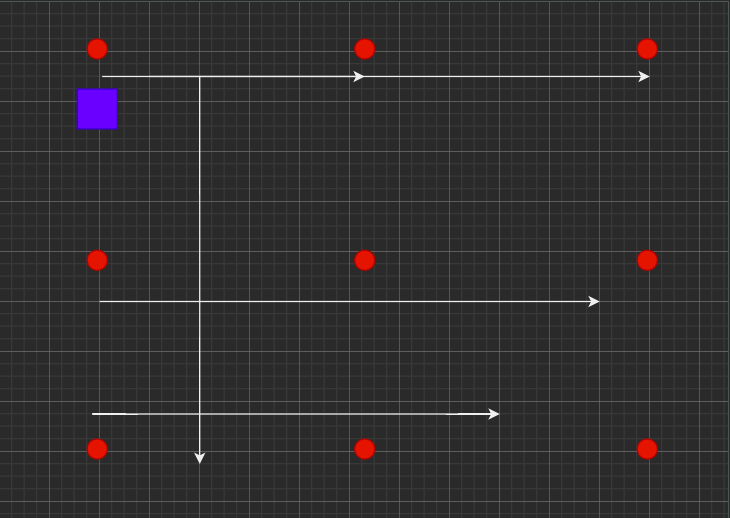
\includegraphics[width=.8\textwidth]{map_poi_test.png}
    \caption{Mapa representando POIs (pontos vermelhos) e \texttt{map-paths} (setas) para o sistema de navegação}
    \label{fig:navigation_map}
\end{figure}

Ao inicializar o sistema de navegação, uma função de navegação deve ser informada. Essa função recebe como parâmetros o mapa do ambiente, a posição atual do robô e sua posição de destino, e deve retornar um caminho (\texttt{Path}) da origem até o destino através dos caminhos seguros do mapa. É permitido que os robôs saiam dos caminhos seguros dentro de um limite que pode ser configurado no componente \texttt{Map}. A função \texttt{find\_route} (\texttt{simulator/systemas/NavigationSystem}) pode ser usada como função que encontra caminhos.

% TODO: Adicionar referência ao projeto do gazebo que usa esse sistema de caminhos
Encontrado um caminho do ponto de origem ao ponto de destino, o componente \texttt{Path} que representa esse caminho a ser seguido é adicionado à entidade. A partir desse ponto o sistema de caminhos (\texttt{PathProcessor}) se encarrega de adicionar velocidade ao robô para que passe por todos os pontos do caminho. Ao chegar no destino, o componente é removido. Caso um caminho não seja encontrado, um evento de erro é adicionado à fila de eventos, para que o controlador do robô (que passou o comando de movimentação) possa tomar a decisão apropriada.

A simulação \texttt{poi\_test} (ver figura \ref{fig:navigation_map}) foi feita para testar o sistema de navegação. Nessa simulação um robô (o quadrado) recebe instruções para ir a alguns POIs (os círculos) em sequência, utilizando o sistema de navegação. Ele segue os caminhos definidos no mapa (as setas). 

Toda vez que uma entidade encontra um caminho até um objetivo, esse caminho encontrado (que pode passar por pontos ainda não mapeados) é incluído ao mapa compartilhado, na tentativa de expandi-lo. Assim, quanto mais as entidades navegam pelo mapa, mais pontos conhecem e mais pontos podem acessar.

\subsection{Sistema de Controle}
\label{sec:scripting}

O sistema de controle (ou sistema de script) foi criado para facilitar o controle e passagem de instruções às entidades da simulação. Ele é especialmente indicado para criar o equivalente a NPCs (\textit{non playable characters}) numa simulação, ou seja, entidades que precisam se movimentar de alguma forma, mas não são o foco da simulação. Esse sistema foi feito para ser extensível por outros sistemas, e funciona baseado em instruções. Na figura \ref{fig:example_annotations}, um dos componentes do robô é \texttt{component\_Script}, que é o componente utilizado pelo sistema de controle. O vetor de strings passados para esse componente é a sequência de instruções que ele vai realizar na simulação, gerenciadas pelo sistema de controle. Esse sistema é reativo e reage à eventos anotados como funções ou como eventos de interesse.

Uma instrução pode ser definida por qualquer sistema, e incluída no sistema de script durante sua inicialização. Elas são implementadas através de funções que aceitem argumentos específicos (detalhes na documentação do projeto), e cujo retorno é o estado do script daquela entidade ao executar a instrução. Por exemplo, na figura \ref{fig:example_annotations} a função \texttt{Go} foi definida pelo sistema de navegação, e as funções \texttt{Grab} e \texttt{Drop} pelo sistema da garra (um atuador que será discutido na Seção \ref{sec:robot_skills}).

Existem 3 estados que um script pode estar ao longo da simulação: \texttt{READY}, \texttt{BLOCKED} ou \texttt{DONE}. \texttt{DONE} significa que todas as instruções do script foram executadas. \texttt{READY} indica que a entidade está pronta para executar a próxima instrução. \texttt{BLOCKED} sinaliza que a entidade está executando alguma ação do script, ou esperando que algo aconteça para poder executar a próxima instrução. Para dar suporte às ações asíncronas, existe uma lista de eventos que o script espera. Toda vez que uma instrução asíncrona é executada, espera-se que o retorno seja o estado \texttt{BLOCKED}, e que tenham sido adicionadas ao componente de script as tags dos eventos que marcam o final da ação sendo executada. O sistema de controle é ativado ao receber um evento com alguma dessas tags, e vai removendo elas da lista de espera do script da entidade apropriada. Quando essa lista fica vazia a entidade é desbloquada (i.e. passa do estado \texttt{BLOCKED} para o estado \texttt{READY}).

Por exemplo, se a entidade $2$ vai executar a instrução \texttt{Go poi}. Essa instrução pode emitir um evento para o sistema de navegação movimentar a entidade $2$ até a coordenada do ponto de interesse "poi". Quando o robô chegar até o ponto de destino, nesse sistema, é emitido um evento \texttt{EndOfPath}. Nesse caso, a função que implementa a instrução \texttt{Go} deve adicionar o evento \texttt{EndOfPath} na lista de espera do script da entidade $2$ e retornar o estado \texttt{BLOCKED}. Passado algum tempo, a entidade $2$ vai chegar até o seu destino, o evento \texttt{EndOfPath} será emitido e capturado pelo sistema de controle, esse evento será removido da lista de espera do script, deixando-a vazia e indicando que a entidade $2$ pode executar a próxima instrução.

Esse sistema de controle foi testado nas simulações \texttt{poi\_test} e \texttt{hospital\_scenario}, com instruções implementadas por diferentes sistemas. O sistema de controle em si só necessita do componente \texttt{Script} e dos eventos para funcionar. Ele desconhece a implementação das instruções passadas em sua inicialização, o que permite grande flexibilidade ao sistema.

O sistema de controle também é capaz de tratar erros. Isso é feito passando um dicionário \texttt{error\_handlers} ao componente \texttt{Script} de uma entidade. Esse dicionário possui tags de erros como chaves e uma ação a ser realizada como valor. Ao receber um erro, o sistema de controle verifica se existe uma ação para aquele erro e a executa caso exista. Se não existir ele tenta realizar uma ação genérica (e.g. panic!) que pode ser configurada. Esse comportamento de tratamento de erros foi testado na simulação \texttt{poi\_test}, onde uma das instruções não retorna um caminho completo até o destino, apenas um caminho parcial que é seguido. É esperado que um sistema que implemente instruções implemente também as ações a serem realizadas em caso de erro da sua instrução e as adicione ao dicionário de erros.

\subsection{Sensores e Atuadores}
\label{sec:robot_skills}

Sistemas que representam sensores e atuadores conferem diferentes habilidades à entidades da simulação. Atuadores podem abstrair componentes inteiros do robô (e.g. garras, plataformas, pinças, etc) e podem ser modulados através de sistemas DES reativos, que reagem à comandos. Sensores por outro lado por terem um comportamento mais constante podem ser também aproximados por sistemas normais. A construção desses sistemas é feita de acordo com requisitos das habilidades do robô, portanto os sistemas implementados e testados são mais como provas de conceito.

Um sistema genérico de sensores foi desenvolvido (\texttt{SensorSystem}). Ele pode ser inicializado com uma frequência e um tipo de sensor (um componente) que tenha uma área de atuação (\texttt{sensor\_range}) e um canal para receber eventos (\texttt{reply\_channel}, um \texttt{simpy.Store}). A ideia é que para cada tipo de sensor dentro da simulação, uma instância desse sistema seria adicionada ao ambiente de simulação, e seria responsável por capturar todas as entidades dentro da área do sensor e enviá-las através de um evento para o sensor de cada entidade através do canal do sensor. Isso abstrai a fase de captura de dados. Um sistema extra que implemente o sensor em si - processamento dos dados e envio de informações - ainda deve ser construído.

Atuadores são mais específicos. A simulação \texttt{hospital\_scenario} implementa um atuador garra, capaz de pegar objetos iterativos e deixá-los em algum outro lugar. Objetos são marcados como interativos com uma anotação no mapa. Para auxiliar o processo de pegar e deixar objetos, que nessa simulação efetivamente remove a entidade interativa da simulação e depois a reconstroi em outro local do mapa, o sistema de gerenciamento de objetos pode ser usado (\texttt{ManageObjects}). O sistema da garra foi usado também para testar a criação de instruções para o sistema de controle, exportando duas instruções.

\subsection{Seer}
\label{sec:seer}

Até o momento não foi mencionado como extrair informações da simulação, e particularmente como visualizar a simulação. Visto que a construção de uma simulação utilizando um diagrama é predominantemente visual, é esperado que a visualização da mesma seja: (1) semelhante ao mapa construído e (2) tão intruitiva quanto construir a simulação. Isso é suportado através do sistema Seer, implementado como um sistema DES. Essa decisão foi tomada para permitir que o simulador seja executado sem qualquer visualização gráfica, por ser uma operação custosa durante a execução da simulação.

\begin{figure}[ht]
    \centering
    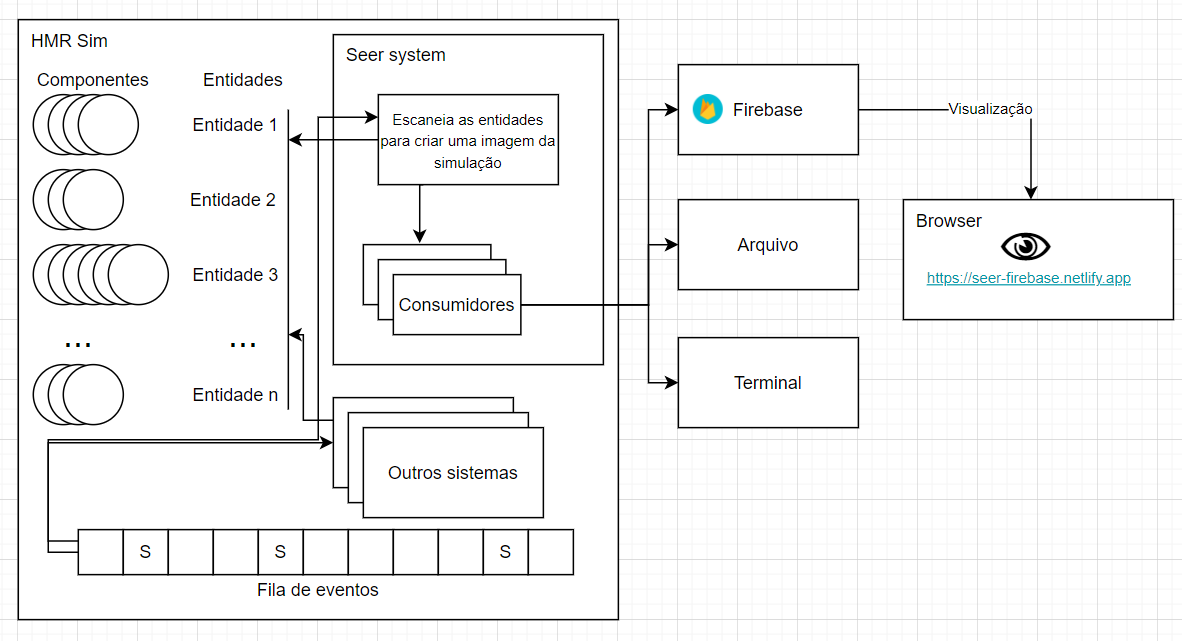
\includegraphics[width=\textwidth]{seer_architecture.png}
    \caption{Esquema da arquitetura do sistema Seer}
    \label{fig:seer_architecture}
\end{figure}

Seer é um sistema opcional como qualquer outro. A figura \ref{fig:seer_architecture} mostra um esquema da arquitetura desse sistema, feito para ser extensível. Ele utiliza os componentes \texttt{Position} e \texttt{Skeleton}, esse segundo sendo utilizado para guardar o estilo das entidades no XML do mapa. A cada evento do Seer (ilustrados na figura \ref{fig:seer_architecture} pelos espaços marcados com 'S' na fila de eventos) o sistema escaneias as entidades e cria uma mensagem que representa uma "fotografia" (e.g. \textit{snapshot}) da simulação naquele ponto. A frequência com que o Seer tira essas fotografias é especificado na inicialização do sistema. 

Criada a mensagem representando o estado da simulação em um ponto ela é colocada numa fila de mensagens. O gerenciador dos consumidores, que executa numa thread separada do simulador, remove as mensagens dessa fila e as passa para uma lista de consumidores. Esses consumidores são funções que vão processar as mensagens, e possivelmente enviá-las para outros locais de armazenamento, como mostrado na figura. Os consumidores são passados para o Seer no momento de sua inicialização, e podem ser criados para atender às necessidades particulares do usuário. 

Um consumidor de destaque, representado na figura pelo caminho que vai até o Firebase e está conectado ao browser é o consumidor do firebase. Esse consumidor utiliza o banco de dados em tempo real do firebase para enviar as mensagens ao firebase. Um programa auxiliar que faz a tradução das mensagens no firebase e reconstroi a simulação é disponibilizado no endereço \url{https://seer-firebase.netlify.app}. Ele tem suporte a múltiplas simulações, e também permite visualizar os logs da simulação (ver figura \ref{fig:dullens_big_contribution}). A visualização da simulação em si utiliza a mesma biblioteca \texttt{jGraph} que a construção do mapa, para manter o máximo de compatibilidade, e pode ser executada passo a passo ou em sequência como um vídeo. As mensagens ficam salvas no banco de dados do Firebase e podem ser vistas depois, permitindo analises posteriores à simulação sem a necessidade de re-executar a simulação toda, um processo que pode ser custoso e demorado. 

Outro sistema que exemplifica a possibilidade de extrair informações da simulação é o sistema \texttt{ClockSystem}, que registra o tempo gasto para simular 1 segundo da simulação e guarda essa informação em um arquivo externo.

\begin{figure}
    \centering
    \begin{subfigure}[b]{0.4\textwidth}
        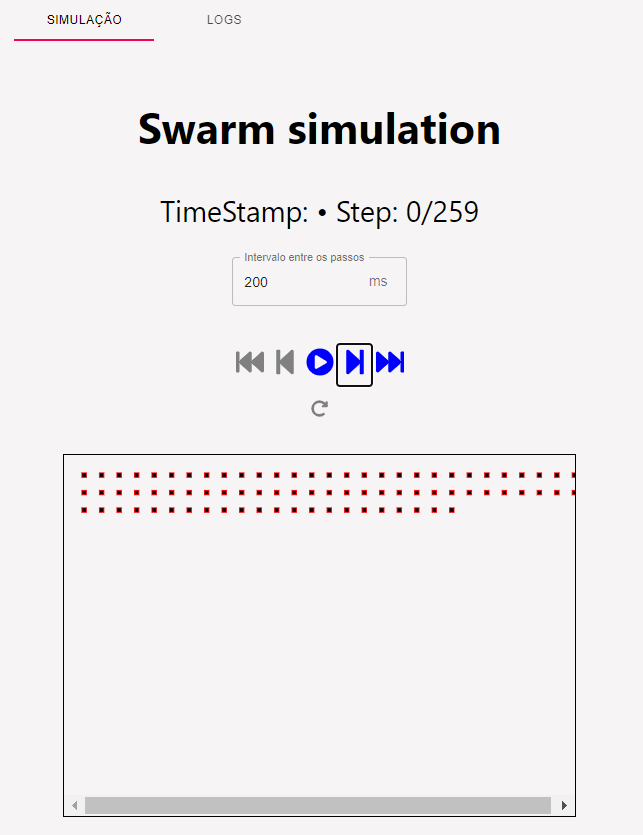
\includegraphics[width=\textwidth]{seer_simulation.png}
    \end{subfigure}
    \hfill
    \begin{subfigure}[b]{0.5\textwidth}
        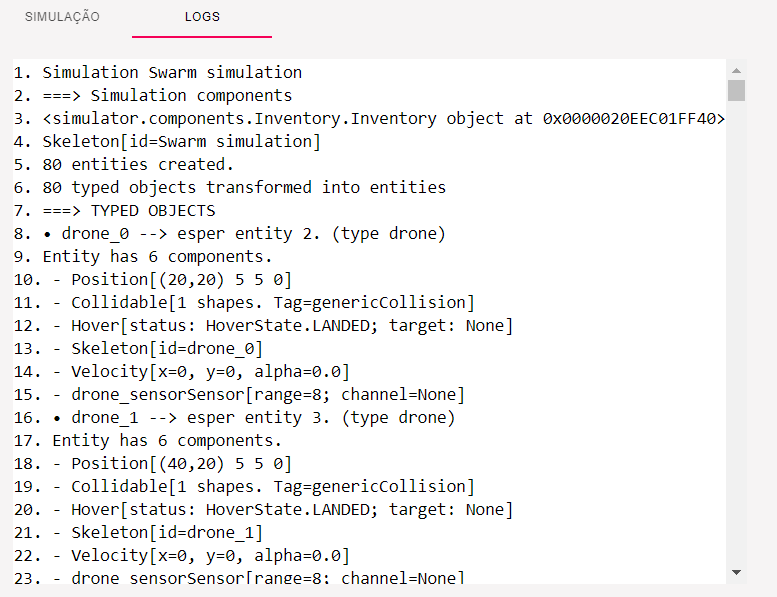
\includegraphics[width=\textwidth]{seer_logs.png}
    \end{subfigure}
    \caption{Visualizador do Seer disponível em \url{https://seer-firebase.netlify.app}}
    \label{fig:dullens_big_contribution}
\end{figure}

\section{Desempenho}
\label{sec:performance}

Um dos objetivos desse projeto é ter um simulador capaz de simular grandes times de robôs (50-200) de maneira eficiente. Para medir o desempenho do simulador nessas condições foi utilizada uma simulação de enxame de drones, aumentando a quantidade de drones de 20 até 200, e marcando quanto tempo demorou o tempo de processamento de 1 segundo da simulação ao longo da simulação. 

A simulação pode ser descrita da seguinte maneira: “Um controlador que conhece configuração para os drones tomarem. Temos uma quantidade grande de drones disponíveis. O controlador decide qual posição na configuração cada drone deve tomar e informa o drone qual sua posição. Cada drone deve tentar movimentar-se até a posição alvo sem bater nos outros drones. Ao chegar em sua posição, deve informar ao controlador e manter sua posição. Se ele bater em outro drone no caminho deve informar ao controlador. O controlador espera a resposta de todos os drones, ou um tempo máximo de 15s antes de encerrar a simulação".

Essa simulação foi construída programaticamente. A posição inicial e a posição final dos drones na simulação com 80 drones é mostrada na figura \ref{fig:drone_swarm}. Essa simulação pode ser vista pelo visualizador do Seer no usuário "simulator".

\begin{figure}
    \centering
    \begin{subfigure}[b]{0.4\textwidth}
        \centering
        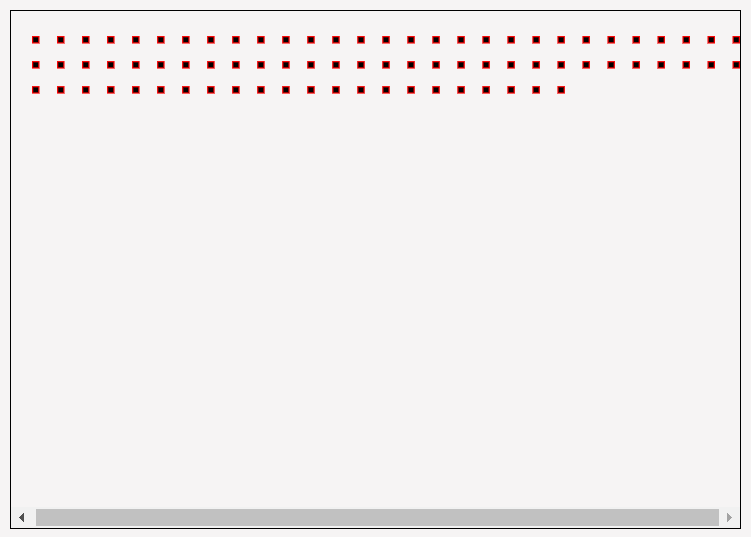
\includegraphics[width=\textwidth]{drone_swarm_init.png}
        \subcaption{Configuração inicial}
    \end{subfigure}
    \hfill
    \begin{subfigure}[b]{0.4\textwidth}
        \centering
        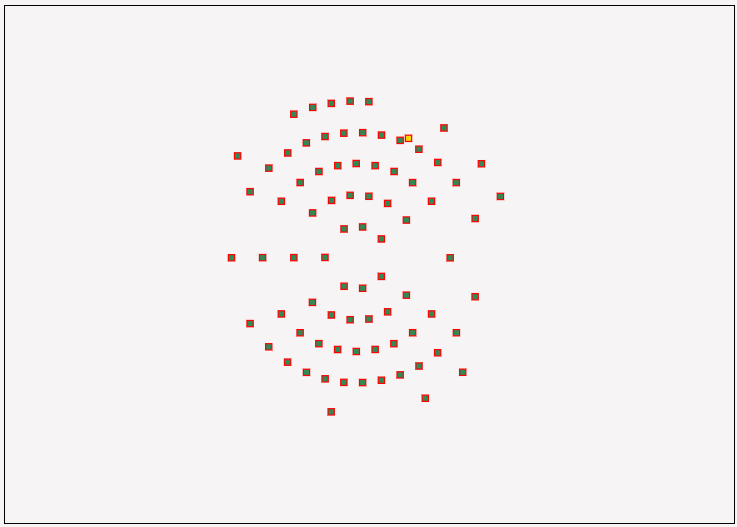
\includegraphics[width=\textwidth]{drone_swarm_end.png}
        \subcaption{Configuração final}
    \end{subfigure}
    \caption{Configurações inicial e final do enxame com 80 drones}
    \label{fig:drone_swarm}
\end{figure}

A tabela \ref{table:performance} mostra um resumo do desempenho do simulador com quantidades diferentes de drones. Tempo simulado é o tempo total da simulação, tempo mínimo e máximo são o menor e maior tempo do relógio necessário para computar 1s de simulação. Média é a média total em segundos do tempo do relógio para se computar 1s de simulação. A diferença no tempo necessário para computar um segundo de simulação está relacionado à posição dos drones ao longo da simulação. Nessa simulação, com 80 drones o tempo da simulação está aproximadamente sincronizado com o tempo do relógio.

\begin{table}
    \begin{tabular}{ccccccc}
        \toprule
        Nº de Drones &  Tempo Simulado &  Min. tempo 1s &  Max. tempo 1s &  Média \\
        \midrule
        20  &                8s &       0.0979s &       0.1778s &  0.1414s \\
        40  &               10s &       0.2700s &       0.3969s &  0.3458s \\
        60  &               20s &       0.4404s &       0.8829s &  0.6042s \\
        80  &               23s &       0.6978s &       1.3350s &  0.9698s \\
        100 &               22s &       0.9491s &       2.3663s &  1.4146s \\
        150 &               25s &       1.7435s &       3.0516s &  2.3176s \\
        200 &               32s &       3.1433s &       4.4711s &  3.7685s \\
        \bottomrule
    \end{tabular}
    \caption{Desempenho do simulador na simulação de enxame de drones por número de drones}
    \label{table:performance} 
\end{table}

A figura \ref{fig:time_process_across} mostra amédia de tempo de relógio necessário para computar 1s de simulação em função da quantidade de drones simulados. Fazendo a aproximação da função do gráfico com regressão quadrática obtemos a função $0.0001x^2+0.0087x-0.0641$, com média de erro relativo de 4.57\%. Usando regressão de expoente o resultado é $0.0018x^{1.4322}$, com erro relativo de 4.23\%. Isso indica que o aumento de entidades nessa simulação acarreta um aumento do tempo da simulação de forma polinomial, com um coeficiente próximo de 2.

A figura \ref{fig:drone_times} mostra como a média de tempo de relógio necessário para computar 1s de simulação muda ao longo da simulação, com números diferentes de drones. É possível observar que independente da natureza dos drones, existe uma tendência de aumento do tempo médio até um pico e depois uma queda até o final da simulação. Isso acontece devido à natureza da simulação. Inicialmente todos os drones estão a uma distância constante (veja figura \ref{fig:drone_swarm}), conforme o controlador assinala posições aos drones eles começam a se movimentar na direção do centro do mapa e ficam mais próximos uns dos outros (ver figura \ref{fig:time_peak}), causando um aumento no tempo de processamento (principalmente devido ao sistema de colisão). Conforme os drones chegam nas suas posições (ver figura \ref{fig:drone_swarm}) o número de entidades ativamente se movendo diminui, e com isso o tempo de processamento médio também. Isso indica que a natureza da simulação afeta diretamente o desempenho do simulador.

\begin{figure}[ht]
    \centering
    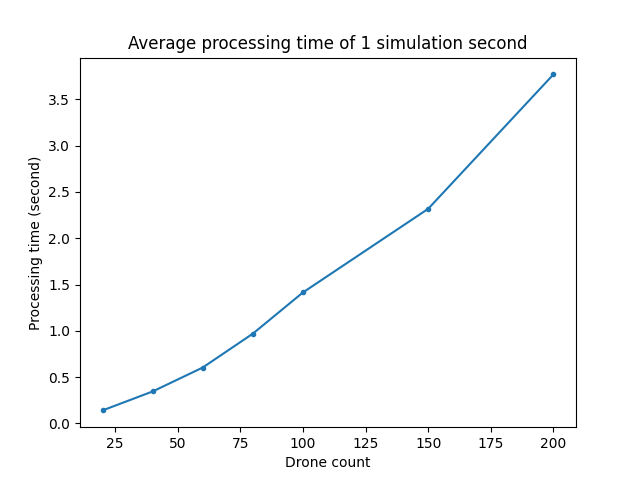
\includegraphics[width=\textwidth]{time_process_1s_across_simulations.png}
    \caption{Tempo para processar 1s de simulação por número de drones}
    \label{fig:time_process_across}
\end{figure}


\begin{figure}
    \centering
    \begin{subfigure}[b]{0.4\textwidth}
        \centering
        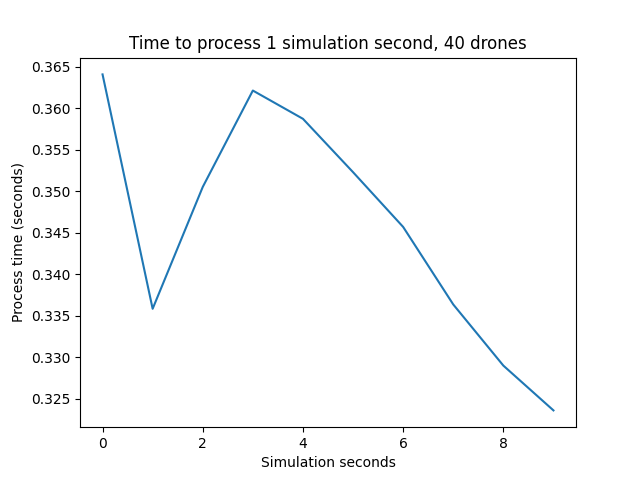
\includegraphics[width=\textwidth]{time_process_1s_simulation_40drones.png}
        \subcaption{40 drones}
    \end{subfigure}
    \hfill
    \begin{subfigure}[b]{0.4\textwidth}
        \centering
        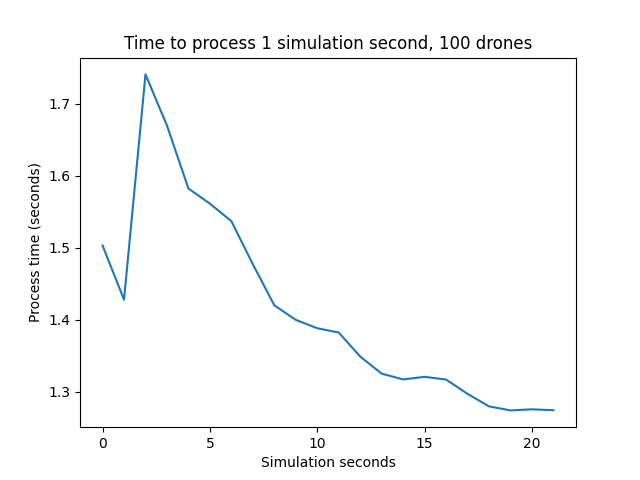
\includegraphics[width=\textwidth]{time_process_1s_simulation_100drones.png}
        \subcaption{100 drones}
    \end{subfigure}
    \begin{subfigure}[b]{0.5\textwidth}
        \centering
        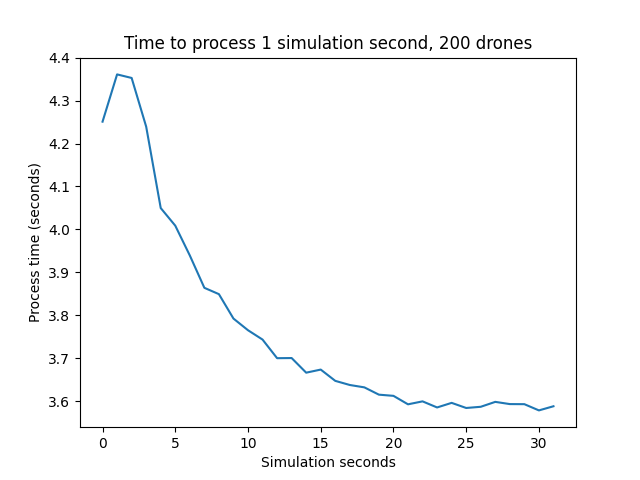
\includegraphics[width=\textwidth]{time_process_1s_simulation_200drones.png}
        \subcaption{200 drones}
    \end{subfigure}
    \caption{Tempo médio para computar 1s de simulação ao longo da simulação com 40, 100 e 200 drones}
    \label{fig:drone_times}
\end{figure}

\begin{figure}[ht]
    \centering
    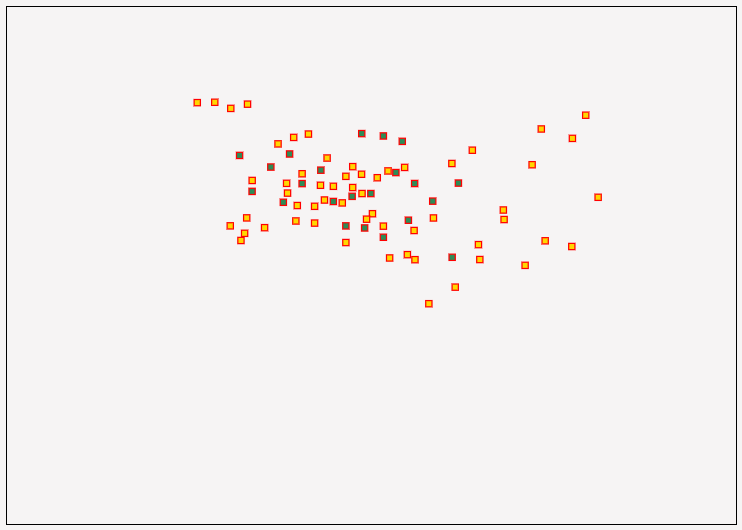
\includegraphics[width=.8\textwidth]{swarm_peak.png}
    \caption{Drones próximos uns dos outros ao longo da simulação. Pontos verdes são drones pairando em sua posição. Pontos amarelos são drones movendo-se para sua posição }
    \label{fig:time_peak}
\end{figure}

\chapter{Testes}
\label{chap:tests}
\label{chapter:testsBdd}
\gab{Destacar aqui duas finalidades - 1 .testar o próprio simulador. 2. Implementar testes automatizados do comportamento de sistemas  utilizam o simulador}

A fim de fazer a verificação e validação do simulador HMR Sim, foi proposto utilizar o Behavior Driven Development. Dessa forma foi sugerido um framework de testes para ajudar no processo. O framework é composto por \del{uma estrutura de pastas, composta pelas especificações das missões na linguagem Gherkin, dos testes dessas missões e por }um conjunto de métodos desenvolvidos para auxiliar na criação e nas assertivas dos cenários.

\section{Estruturação dos Testes}
\label{sec:estruturacaoTestes}
\begin{figure}
\centering
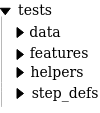
\includegraphics[scale=0.8]{imagens/estrutura_pasta.png}
\caption{Estrutura de pasta dos testes.} 
\label{fig:estruturaPasta}
\end{figure}

A parte de teste é dividida em quatro pastas:
\begin{itemize}
    \item \textbf{features}: Contém a descrição dos cenários e passos de cada funcionalidade. Cada funcionalidade está descrita em um arquivo .feature, que faz uso da linguagem Gherkin. Os arquivos das Features são estruturados da seguinte forma:
    \begin{itemize}
        \item Os passos Given são responsáveis por fazer a montagem do cenário, por exemplo, instanciar uma simulação, associar um mapa à simulação, adicionar sistemas, criar POIs (pontos de interesse), criar caminhos, adicionar componentes ao robô.
        \item Os passos When são responsáveis por executar a simulação, chamando o método run da simulação.
        \item Os passos Then são responsáveis por fazer as assertivas, verificando se a simulação fez o que era esperado.
    \end{itemize}
    \item \textbf{step\_defs}: Os arquivos dessa pasta possuem a montagem dos passos da simulação, a execução da simulação e as assertivas. Cada arquivo da pasta step\_defs é relacionado com um arquivo .feature da pasta features e todos os passos presentes no .feature devem estar presentes também no arquivo de testes, conforme mostra a figura \ref{fig:singleStaticRobotF} e a figura \ref{fig:singleStaticRobotT}. 
No início dos arquivos ocorre a instanciação da simulação e dos helpers (ScenarioCreationHelper e AssertionHelper), que serão usados nos passos given, when e then.
    \item \textbf{helpers}: A pasta possui duas classes de métodos auxiliares. A primeira classe, a ScenarioCreationHelper, possui métodos para auxiliar na criação dos cenário, sendo alguns desses métodos: add\_component (adiciona um componente em uma entidade), create\_path (cria um caminho que parte de uma entidade e passa por diferentes pontos no mapa), add\_goto\_position\_event (adiciona um evento na event store para que o robô se movimente até uma determinada posição), add\_poi (adiciona um ponto de interesse na mapa). A segunda classe, a AssertionHelper, possui métodos para auxiliar nas assertivas, contendo mensagens de erros mais completas. Sendo alguns desses métodos: have\_collided (verifica se uma entidade colidiu com outra entidade), is\_in\_poi (verifica se o centro de uma entidade está posicionado em um ponto), approximated (verifica se um robô X se aproximou de uma entidade Y).
    
\begin{figure}
\centering
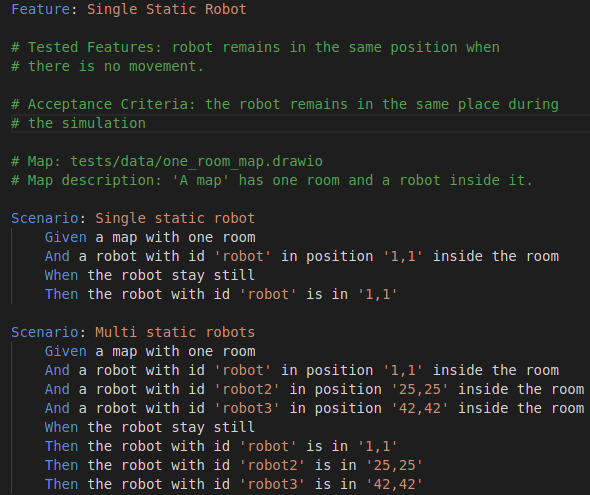
\includegraphics[scale=0.5]{imagens/single_static_robot_feature.png}
\caption{Arquivo single\_static\_robot.feature.} 
\label{fig:singleStaticRobotT}
\end{figure}

\begin{figure}
\centering
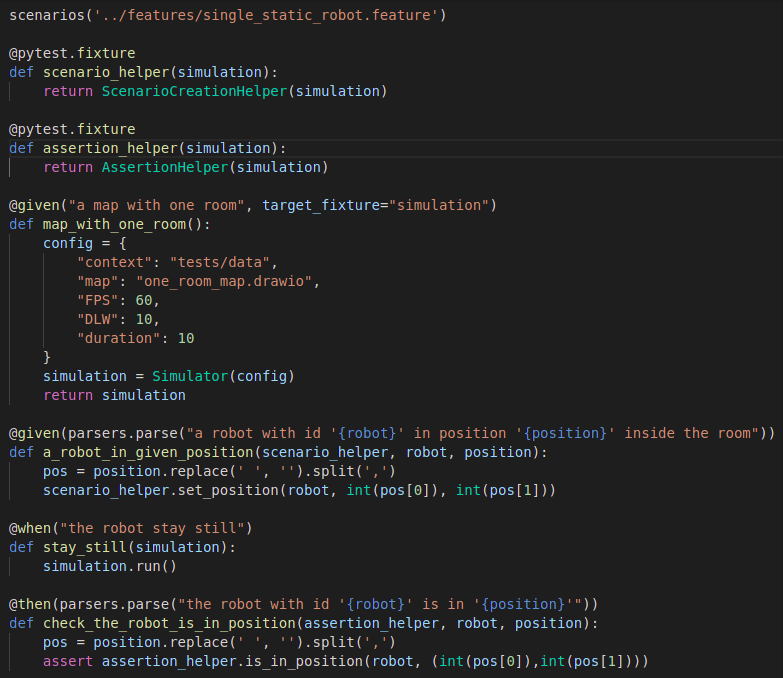
\includegraphics[scale=0.5]{imagens/test_single_static_robot.png}
\caption{Arquivo de teste test\_single\_static\_robot.py.} 
\label{fig:singleStaticRobotF}
\end{figure}
    
    \item \textbf{data}: Possui os mapas necessários para a criação de uma simulação. Os mapas são feitos utilizando a ferramenta draw io.

\end{itemize}
\section{Capacidades e Limitações}
\label{sec:limitacoesTeste}
\gab{Mover a discussão sobre as limitações para o final do capítulo. Primeiro o leitor deve ter uma idéia do que é capaz para depois saber as limitações.}
A princípio, é possível verificar:
\begin{itemize}
    \item Posições finais de entidades;
    \item Informações salvas em componentes que são capturadas durante a execução dos sistemas.
\end{itemize}

Não é possível verificar:
\begin{itemize}
    \item Informações que não fazem parte do estado final  da simulação, a não ser que essa informação tenha sido gerada por um dos sistemas e tenha sido guardada em algum componente que possa ser acessado ao término da execução;
    \item Informações que mudam a cada vez que a simulação é executada, ou seja, não é possível testar informações que não são possíveis de se reproduzir.
\end{itemize}

Nos testes são feitos os seguintes tipos de verificações e existem as seguintes limitações:
\begin{itemize}
    \item \textbf{Robot Displacement}: é verificado se um robô foi até a posição requisitada (posição final do robô), mas não verifica o caminho que ele percorreu.

    \item \textbf{Scripted Commands}: são verificadas se determinadas entidades estão na posição ou ponto de interesse (POI) correto. Um dos cenários, testa se um medicamento (pickable) foi deixado em uma determinada posição. No entanto, só se verifica a posição final dele. Para verificar posições intermediárias é necessário guardar em um componente as informações dos locais que o robô deixou o pickable.

    \item \textbf{Collision}: é verificado se um robô colidiu com outra entidade, para isso é testado se o identificador da entidade colidida está presente na lista de colisões do robô, guardada no componente CollisionHistory. Uma limitação dessa abordagem é que só é guardado a última colisão entre o robô e uma determinada entidade.

    \item \textbf{Seer}: é possível acessar as mensagens geradas pelo Seer, mas é necessário guardá-las em um componente ou em arquivo para depois acessar essas mensagens e testá-las. No entanto, é trabalhoso testar se todos os logs estão no formato esperado, e se a formatação das mensagens muda, é preciso mudar as assertivas. Por conta disso, o teste do Seer verifica apenas se o arquivo gerado possui pelo menos uma linha no formato json, e se essa primeira linha possui uma chave com o nome “timestamp”.
    
    \item \textbf{Camera}: é possível verificar se uma ou mais entidades foram detectadas por um robô que possui o componente Camera. No entanto, uma das limitações é que a câmera guarda apenas uma detecção de um alvo (a última adicionada), por exemplo, se detectar uma pessoa duas vezes, guarda apenas a última detecção.

    \item \textbf{Approximation}: é verificado se o robô se movimentou até a pessoa detectada, sendo essa informação guardada em um componente do tipo ApproximationHistory. No momento não é possível fazer duas aproximações porque a Câmera é removida quando a primeira aproximação ocorre e o ApproximationHistory só guarda informações de uma aproximação.
\end{itemize}

Para verificar passos intermediários, por exemplo, verificar os pontos que o robô parou durante a simulação, é necessário guardar a informação em uma lista para depois acessá-la na hora de fazer a verificação.

Uma outra limitação está presente nos métodos de assertivas (tests/helpers/AssertionHelper.py): A maioria dos métodos verifica apenas o caso verdadeiro, caso contrário lança um erro (raise AssertionError). Então para verificar os casos falsos seria necessário fazer modificações nos métodos ou criar novos.

\section{Criando uma Feature utilizando o HMR Sim e princípios do BDD}
\label{sec:featureBDD}
Como parte da validação do simulador, foi feito um sistema a partir do zero, desde a criação dos cenários e testes até a implementação de novos mapas, componentes e sistemas.

Utilizando o Sistema de Aproximação proposto, o robô é capaz de percorrer um caminho procurando uma pessoa, para isso utiliza um componente do tipo câmera, e se essa pessoa estiver no campo de visão da câmera, ele se aproxima dela. 

\subsection{Sistema de Detecção e de Aproximação}
\label{sec:sistemaAprox}
A lógica do sistema de aproximação foi dividida em duas partes. A primeira parte é a responsável por detectar uma entidade solicitada utilizando o CameraProcessor. Já a segunda parte é feita através do sistema de aproximação (ApproximationDESProcessor) e é a responsável por navegar até a pessoa que foi detectada.

A implementação do sistema da câmera foi feita utilizando um sistema já implementado anteriormente, o Sensor System.

A cada iteração, o SensorSystem verifica se existem entidades próximas do sensor. Neste caso, o sensor que será passado como parâmetro é um componente do tipo câmera. Se existirem entidades próximas, o SensorSystem envia um evento contendo um vetor de entidades próximas  para o reply chanel da câmera. Essa etapa é feita utilizando um sistema Publisher/Subscriber, no qual o SensorSystem (Publisher) envia informações 
para uma câmera que fica esperando por essas informações (Subscriber).

Nessa parte entra um segundo sistema, o CameraProcessor, que fica esperando receber essas informações que foram enviadas para o reply chanel da câmera. Esse processador recebe como parâmetro uma câmera e o identificador da entidade que será detectada. Assim que recebe as informações de entidades próximas, o processador compara se uma dessas entidades detectadas era o alvo. Se a entidade detectada for igual ao alvo,essa informação é adicionada à lista de entidades detectadas da câmera e também é enviado um evento avisando sobre a detecção.

Para que o sistema de detecção funcione é necessário:
\begin{itemize}
    \item Adicionar ao robô um componente do tipo Câmera; (colocar o código da função auxiliar);
    \item Iniciar um SensorSystem passando essa câmera como parâmetro e adicionar esse sensor aos DES Systems;
    \item Adicionar um sistema para processar os eventos da câmera.
\end{itemize}

A segunda e última parte do sistema de aproximação é responsável por receber o evento do CameraProcessor que avisa sobre a detecção e a partir disso, o robô se locomove até a entidade detectada. Para fazer a aproximação, o ApproximationDESSystem envia um outro evento do tipo GotoPosEvent que será recebido pelo sistema de navegação, que já foi implementado anteriormente.

Para utilizar esse sistema é necessário:
\begin{itemize}
    \item Adicionar as habilidades de navegação, de detecção de entidades e de aproximação;
    \item Adicionar uma câmera ao robô; 
    \item Adicionar um processador para que o robô procure pela pessoa.
\end{itemize}

\subsection{Criando as funcionalidades de detecção e aproximação utilizando princípios do BDD}
\label{sec:criandoFunc}
O passo inicial antes de implementar as funcionalidades foi a realização dos testes. 

Primeiro foram feitos os testes e a implementação do sistema da Câmera, pois o sistema de aproximação depende dele. Para isso, foram definidos quatro cenários no arquivo camera.feature utilizando a linguagem Gherkin. A figura \ref{fig:cameraFeat} mostra a definição do primeiro cenário.

\begin{figure}
\centering
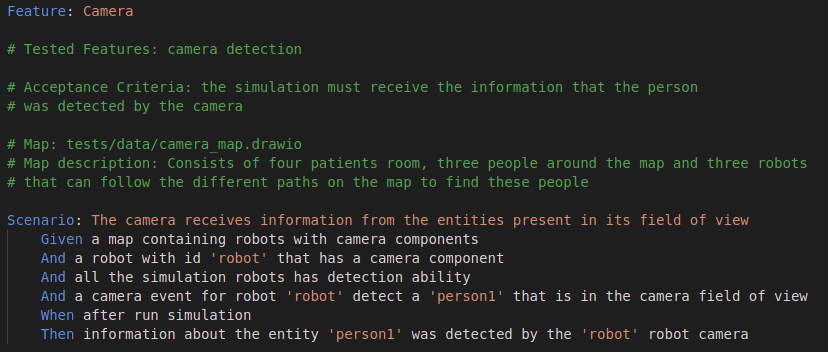
\includegraphics[width=\textwidth]{imagens/cameraFeature.png}
\caption{Definição do primeiro cenário da feature Camera.} 
\label{fig:cameraFeat}
\end{figure}

Depois de descrever os cenários, foi feito um mapa, utilizando o draw io, contendo quartos de pacientes, robôs, pessoas, rotas e pontos de interesse (POIs) para o robô se locomover, conforme mostra a figura \ref{fig:mapaApprox}.

\begin{figure}
\centering
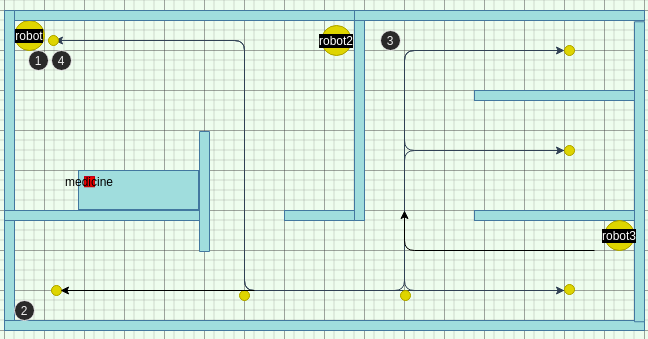
\includegraphics[width=\textwidth]{imagens/mapaApprox.png}
\caption{Mapa dos cenários de detecção e de aproximação.} 
\label{fig:mapaApprox}
\end{figure}

Logo após, foi feita a criação de todos os passos necessários para implementar o cenário da Feature e verificar se tudo ocorreu conforme o esperado, no arquivo test\_camera.py. Nessa etapa é instanciada a simulação e os métodos auxiliares, e também é adicionada a câmera e todos os sistemas necessários, conforme mostra a figura \ref{fig:testCamera}. No entanto, os testes ainda não passam nessa etapa, pois o sistema ainda não foi implementado.

\begin{figure}
\centering
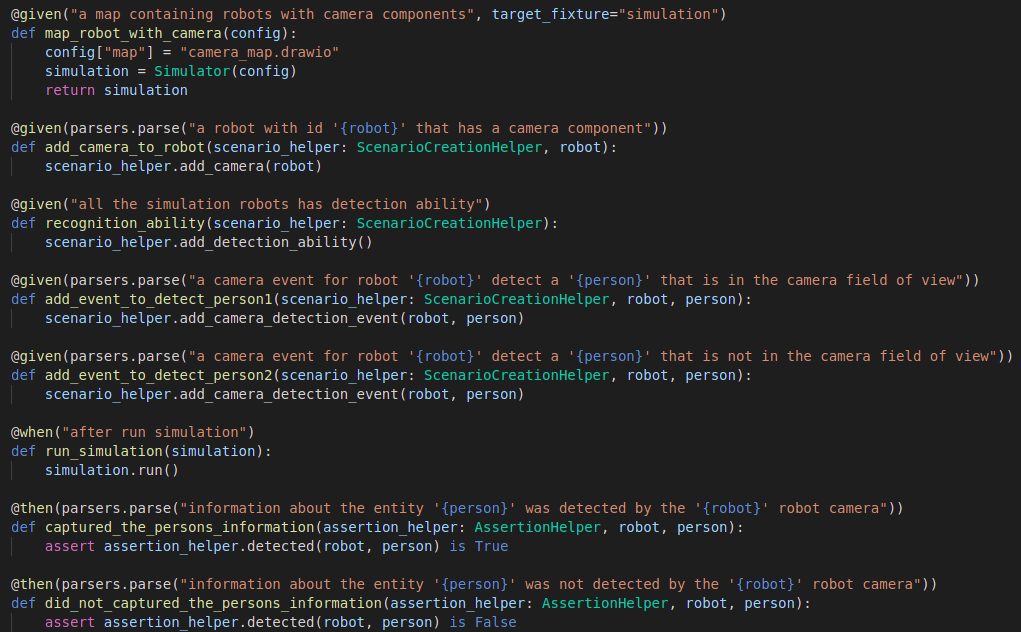
\includegraphics[width=\textwidth]{imagens/testCamera.png}
\caption{Arquivo de teste test\_camera.py.} 
\label{fig:testCamera}
\end{figure}

Em seguida, foi feita a implementação do processador da câmera, o CameraProcessor, que verifica se a câmera detecta um determinado alvo, conforme descrito mais acima. Nessa etapa também é criado um componente do tipo Camera \ref{fig:cameraComp} que herda da classe Component.

\begin{figure}
\centering
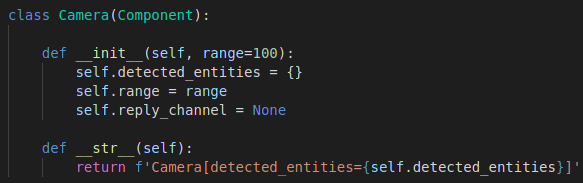
\includegraphics[scale=0.5]{imagens/cameraComp.png}
\caption{Novo componente criado: Camera.} 
\label{fig:cameraComp}
\end{figure}

Retornando aos testes, foi implementado os métodos auxiliares para adicionar o componente de câmera ao robô, para iniciar e adicionar o SensorSystem e para adicionar um processador para receber os eventos de detecção da câmera. Também foi feito um método de assertiva para verificar se ocorreu a detecção.

\begin{figure}
\centering
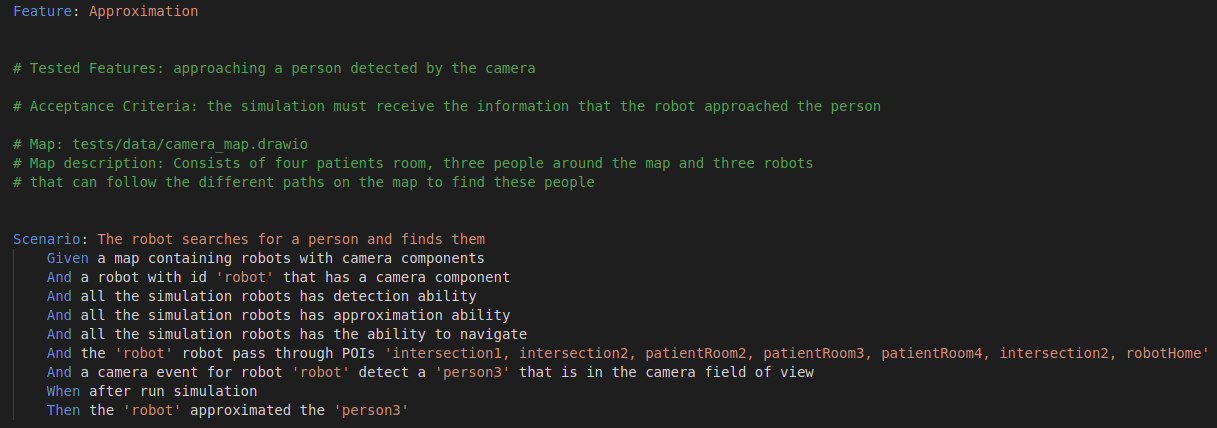
\includegraphics[width=\textwidth]{imagens/approxFeat.png}
\caption{Definição do primeiro cenário da feature Approximation.} 
\label{fig:approxFeat}
\end{figure}

Depois de implementado o sistema de detecção, foi feito o sistema de aproximação, seguindo os mesmos passos descritos acima. Primeiro foram definidos os cenários no arquivo approximation.feature, conforme mostra a figura \ref{fig:approxFeat} e depois foi feita a implementação dos testes no arquivo test\_approximation.py, conforme mostra a figura \ref{fig:Appr1} e a continuação dela \ref{fig:Appr2}. 

\begin{figure}
\centering
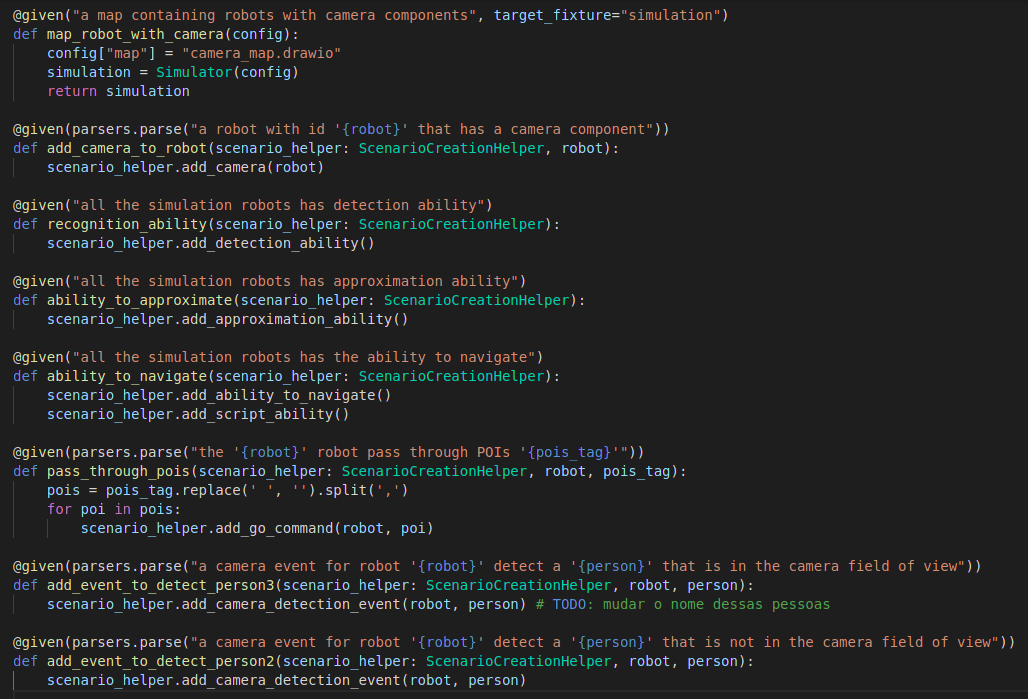
\includegraphics[width=\textwidth]{imagens/Appr1.png}
\caption{Arquivo de teste test\_approximation.py.} 
\label{fig:Appr1}
\end{figure}

\begin{figure}
\centering
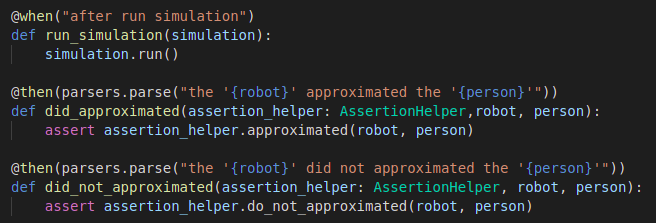
\includegraphics[width=\textwidth]{imagens/Appr2.png}
\caption{Continuação do arquivo de teste test\_approximation.py.} 
\label{fig:Appr2}
\end{figure}

O arquivo de mapa usado é o mesmo do sistema da câmera \ref{fig:mapaApprox}. 
Por fim, foi feita a implementação do sistema de aproximação, que recebe um evento de Detected e envia um evento para o Navigation System para que o robô vá até a posição da entidade detectada. Nessa etapa, é criado um componente do tipo ApproximationHistory para guardar informações sobre a aproximação. 

Também foram implementados métodos auxiliares para montar e validar os cenários de aproximação: um método para adicionar a  habilidade de aproximação e métodos de assertiva para verificar se aproximou da pessoa.

\section{Resultados dos Testes}
\label{sec:testResults}
Para executar os testes foi executado o comando \textit{pytest}, para obter o tempo de execução de todos os cenários, do maior tempo para menor, foi utilizado o comando \textit{pytest --durations=0} e para obter o relatório de cobertura em html, foi executado o comando \textit{pytest --cov-report=html --cov=simulator tests/}.

\begin{figure}
\centering
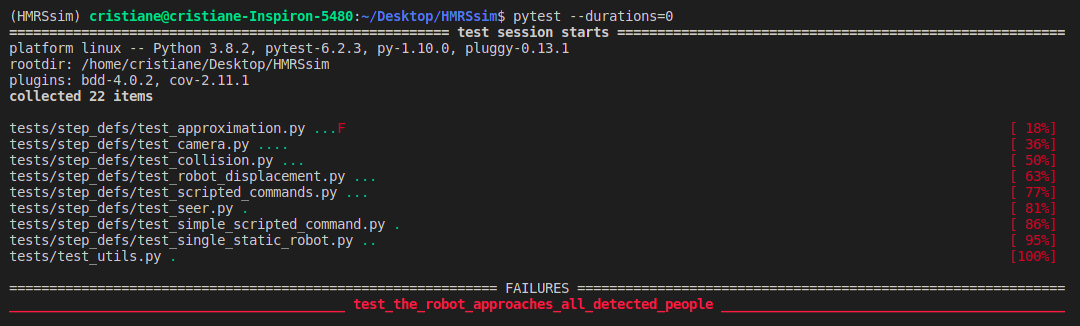
\includegraphics[width=\textwidth]{imagens/testResults.png}
\caption{Resultados do pytest.} 
\label{fig:testResults}
\end{figure}

\begin{figure}
\centering
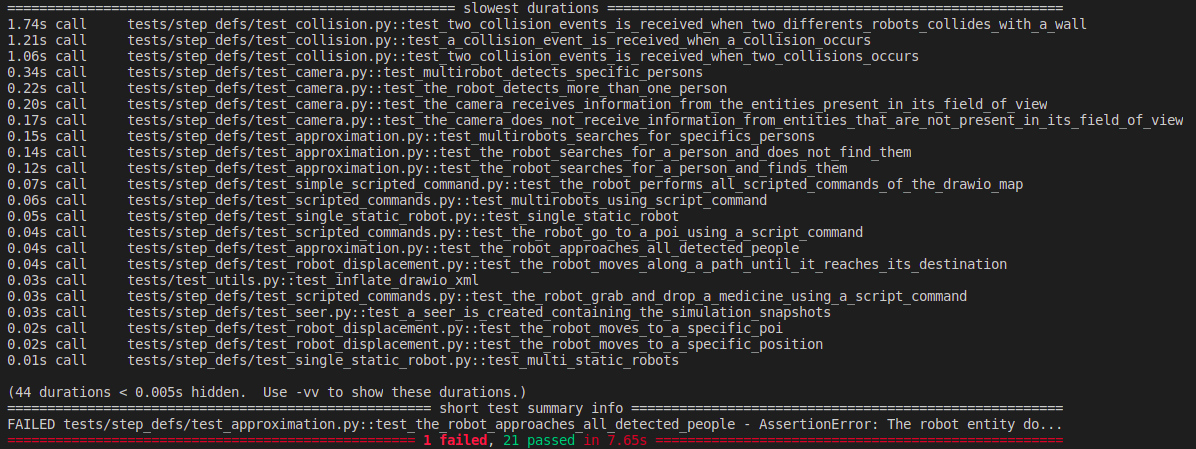
\includegraphics[width=\textwidth]{imagens/timeResults.png}
\caption{Resultados de tempo de execução do pytest.} 
\label{fig:timeResults}
\end{figure}

A figura \ref{fig:testResults} mostra o resultado da execução do pytest para todos os cenários citados abaixo. Pela imagem pode-se observar que todos os cenários estão passando, com exceção do último cenário do test\_approximation.py. Em relação a falha desse teste, uma observação pode ser feita: é possível detectar várias pessoas, conforme mostra o último cenário da \textit{feature Camera}, mas só é possível fazer uma aproximação, que será feita até a primeira entidade detectada.

Um ponto que pode ser observado é o tempo gasto para executar os testes da colisão, que é o maior de todos, conforme mostra a figura \ref{fig:timeResults}.

Da forma que o cenário foi implementado, o robô sai de um ponto inicial e se movimenta por um caminho determinado até colidir com a parede. O robô fica parado nessa parede até o final da simulação e durante todo esse tempo são enviados eventos dizendo que está ocorrendo a colisão.

O sistema de colisão (CollisionProcessor) é um sistema mais custoso que fica ativo durante toda a simulação verificando se ocorreu colisões entre as entidades. Para cada entidade que possui os componentes Collidable, Position, Velocity é verificado se ocorreu uma colisão com cada uma das outras entidades do mapa que possuem os componentes Collidable, Position, ou seja, é uma interação dentro de outra interação. No entanto, o que está causando o gargalo não é essa interação, mas sim a função collide, que é responsável por verificar se uma forma está colidindo com outra. Essa função é chamada dentro de outra função, a checkCollide (simulator/systems/CollisionProcessor.py). Para tentar diminuir o tempo de execução, algumas modificações foram feitas pelo Giovanni (como citar ele?). A imagem X, mostra o tempo de execução após as mudanças feitas no sistema de colisão.

\begin{figure}
\centering
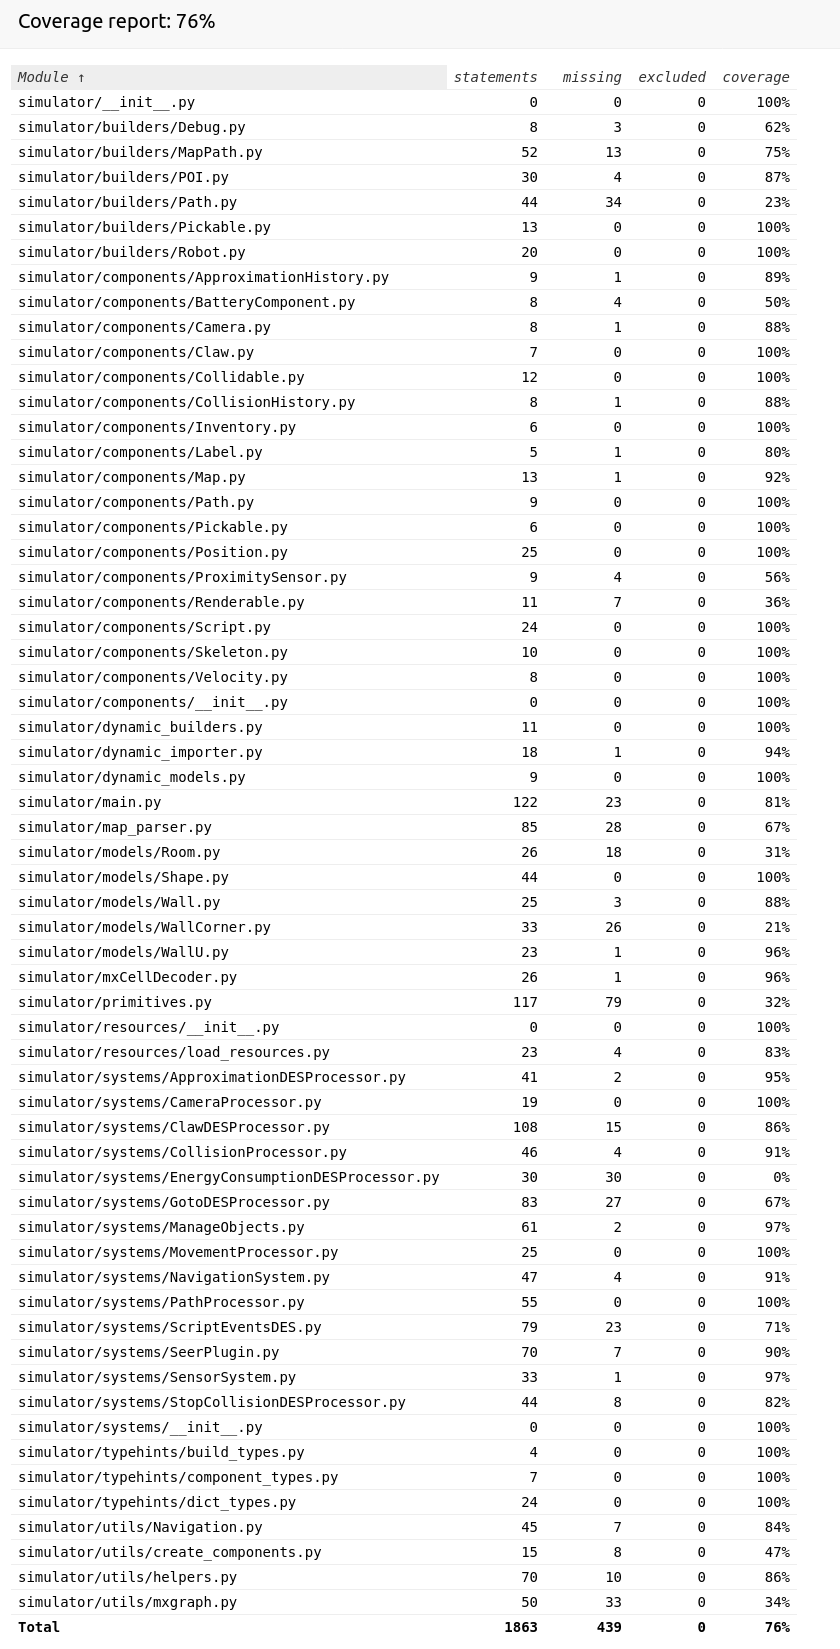
\includegraphics[scale=0.4]{imagens/coverage.png}
\caption{Cobertura dos testes.} 
\label{fig:coverage}
\end{figure}

A cobertura total dos testes ficou em 76\%, conforme mostra a figura \ref{fig:coverage}.
O sistema EnergyConsumptionDESProcessor está com a cobertura em 0\% porque ainda não foi terminado e não possui nenhum cenário de teste. No entanto, o sistema tem potencial e pode ser continuado em trabalhos futuros.

No geral, os cenários de teste usam todas as principais funcionalidades do sistema, conforme mostrado pelo coverage.

\subsection{Single Static Robot}
\label{sec:singleStaticRobot}
É composto por dois cenários. No primeiro cenário (Single static robot), o robô com id ‘robot’ está em uma posição 1,1 no mapa e ao executar a simulação, esse robô deve permanecer parado, pois não foi enviada nenhuma instrução para o robô se movimentar. Portanto, no final, o robô deve estar na posição 1,1.

O segundo cenário (Multi static robots) conta com multi-robôs, cada um numa posição diferente e todos esses robôs devem permanecer parados até o final da execução, pois nenhuma instrução foi dada.

Todos os dois cenários passam, pois todos os robôs permanecem na mesma posição, conforme o esperado.

\subsection{Simple Scripted Command}
\label{sec:simpleScriptedCommand}
É composto por um cenário (the robot performs all scripted commands of the drawio map) no qual o robô lê uma lista de comandos que foram adicionados a ele pelo edit data no drawio: [["Go medRoom", "Grab medicine", "Go patientRoom", "Drop medicine"], 0]. É esperado que o robô vá até a sala de medicamentos (medRoom), pegue o medicamento ‘medicine’ presente nesta sala e depois vá até a o quarto do paciente (pacientRoom) e deixe este medicamente lá. 

O teste passa para esse cenário, pois o robô segue todo o caminho esperado e deixa o medicamento no local correto.

\subsection{Scripted Commands}
\label{sec:scriptedCommands}
O teste é composto por três cenários. No primeiro (The robot Go to a POI using a script command) é verificado se o robô foi até o quarto de medicamentos usando o comando Go. No segundo (The robot grab and drop a medicine using a script command) é verificado se o robô deixou o medicamento no quarto do paciente utilizando os comandos Grab e Drop. No terceiro cenário (Multi-robots using script command) é testado se dois robôs realizam determinados comandos de forma paralela, o primeiro robô deixa um medicamento no quarto do paciente e o segundo robô vai até o quarto do paciente. Os cenários descritos utilizam o sistema de comandos (ScriptEventDES.py) e os comandos Go, Grab e Drop.

Os testes estão passando para todos os cenários descritos acima, pois os robôs seguem corretamente todos os comandos solicitados.

\subsection{Robot Displacement}
\label{sec:robotDisplacement}
O teste é composto por três cenários, no qual cada cenário descreve uma forma diferente de se locomover. Utilizando cada uma dessas três formas, o robô deve parar no mesmo ponto. No primeiro cenário (The robot moves along a path until it reaches its destination), a locomoção é feita através de uma seta (type: Path) que sai do robô e vai até um determinado destino. No segundo cenário (The robot moves to a specific Position), o robô recebe um comando para ir até uma posição (x, y). Já no terceiro cenário (The robot moves to a specific POI), o robô recebe um comando para se locomover até um POI (ponto de interesse).

Os três testes passam, pois o robô para no mesmo ponto de destino independente da forma de locomoção e da rota utilizada.

\subsection{Collision}
\label{sec:collision}
Existem três cenários para testar colisões simples. No primeiro cenário (A collision event is received when a collision occurs), o robô colide com uma parede e recebe uma notificação da ocorrência da colisão. No segundo cenário (Two collision events is received when two collisions occurs), o robô colide com duas paredes diferentes e recebe a notificação da ocorrência das duas colisões. No terceiro cenário (Two collision events is received when two differents robots collides with a wall), é testado se dois robôs colidem com uma parede e se  recebem a notificação de colisões de forma separada.

Todos os testes passam, pois os robôs recebem a notificação da colisão com a parede.

\subsection{Camera}
\label{sec:camera}
O teste é composto por quatro cenários. O primeiro cenário (The camera receives information from the entities present in its field of view) é responsável por  testar se a câmera detectou uma determinada entidade que estava no campo de visão dela. O segundo cenário (The camera does not receive information from entities that are not present in its field of view) é responsável  por testar se não foi detectada uma determinada entidade que não estava no campo de visão da câmera do robô. O terceiro cenário (Multi-robot detects specific persons) é responsável por testar se multi-robôs detectaram determinadas entidades que estavam em seu campo de visão. Já o último cenário (The robot detects more than one person) é responsável por verificar se um robô é capaz de detectar mais de uma pessoa que esteja em seu campo de visão.

Todos os testes passam, pois só são detectadas as entidades que estão no campo de visão da câmera e a funcionalidade serve para um cenário com multi-robôs.

\subsection{Approximation}
\label{sec:approximation}
O teste é composto por quatro cenários. No primeiro cenário (The robot searches for a person and finds them), o robô procura por uma pessoa usando uma câmera e assim que essa pessoa é detectada, o robô se aproxima dela. No segundo cenário (The robot searches for a person and does not find them), o robô procura por uma pessoa, mas não a encontra e logo, ele não se aproxima dela. No terceiro cenário (Multi-robots searches for specifics persons), é testado se mais de um robô com a capacidade de detectar outras entidades, se aproximam das entidades detectadas. No último cenário (The robot approaches all detected people), o robô procura por duas pessoas que estão no campo de visão dele e tenta se aproximar delas.

Os três primeiros testes passam, pois os robôs só se aproximam das entidades detectadas. Já o último teste falha, pois da forma que ocorreu a implementação do ApproximationDESProcessor só é possível fazer uma aproximação.

\subsection{Seer}
\label{sec:seer}
Foi feito um cenário básico (A seer is created containing the simulation snapshots) para testar o funcionamento do sistema Seer, que é responsável por obter snapshots da simulação. O teste cria um cenário simples de movimentação e adiciona o Seer para obter os snapshots. Os resultados obtidos serão salvos em um arquivo seer\_report.txt e depois será verificado se esse arquivo gerado contém os logs. No momento, para testar se o arquivo está correto, é verificado se a primeira linha dele possui um dicionário com uma chave chamada timestamp.

O teste feito passa,  pois o snapshot é gerado corretamente pelo sistema do Seer.

\section{Comparar os problemas apontados e como você tentou resolver eles}
\label{sec:problemasApontados}
Um dos problemas relatados pelos desenvolvedores que utilizam simuladores é a mudança constante nas APIs e a falta de documentação, principalmente em relação a essas mudanças.

Este problema também foi observado durante o desenvolvimento dos testes do HMRS sim e ocorria da seguinte forma: Era gasto um certo tempo para entender como funcionavam todos os parâmetros, sistemas e componentes necessários para fazer funcionar um determinado sistema e depois de entender o funcionamento, eram feitos os testes e eles passavam. No entanto, como a ferramenta estava em constante mudanças, quase toda vez que ocorria um pull da branch dev, todos os testes quebravam por conta de mudanças na forma que eram chamados determinados métodos (mudanças na API). Depois de quebrar os testes, era necessário procurar essas mudanças e os erros que estavam acontecendo para refazer os testes. 

As mudanças constantes na API causaram bastante retrabalho. O que ajudou bastante nessa parte foi que o desenvolvedor da ferramenta sempre ajudava quando entrava em contato com ele, caso contrário, não seria possível aplicar o bdd no projeto.

O que teria ajudado e o que pode ajudar em trabalhos futuros: 
\begin{itemize}
    \item Ter uma interface mais fixa ou ter uma comunicação mais clara da ocorrência de mudanças na interface.
    \item Executar os testes antes de dar um commit.
    \item Uma documentação mais completa e atualizada com todas as mudanças feitas na interface.
\end{itemize}

Outro problema relatado pelos desenvolvedores é não ser possível executar os testes sem desabilitar a Interface Gráfica. Também foi observado este problema no desenvolvimento de testes do HMR Sim quando a parte gráfica era acoplada com o restante do código. Quando estava acoplado, foi gasto semanas e esforço tentando construir os testes e mesmo assim não foi possível, principalmente por causa de dificuldades ao configurar a simulação e executar com a parte gráfica, sendo que uma das dificuldades relatadas é saber a hora de término da execução e fechar o simulador sem ser de forma manual.

Os testes começaram a serem feitos quando ocorreu a separação da parte gráfica do restante do código, assim foi possível verificar de forma mais simples diferentes variáveis e informações da simulação somente pelo código. Se não tivesse ocorrido essa separação, também não teria sido viável fazer a automação dos testes.

Outros aspectos que eram apontados pelos desenvolvedores como um problema era a dificuldade de executar a simulação sem intervenção manual e não ter uma terminação clara da simulação. No entanto, a arquitetura do simulador desenvolvido permite que a simulação funcione sem ser necessário a interação manual com uma interface gráfica e a simulação segue um número de passos limitados, sendo possível saber quando ela termina. Dessa forma, o HMR sim não possui esses dois problemas relatados e isso acaba facilitando a construção de testes e a automação deles.

A dificuldade na construção de cenários e ambientes também foi um problema relatado. Para contornar essa dificuldade foi proposto e desenvolvido um conjunto de métodos auxiliares para auxiliar na construção dos cenários e na realização das assertivas.



% \chapter{Evaluation}
% \label{chap:evaluation}
% \input{parts/evaluation}
% %\input{end/evaluation}

% \chapter{Related Work}
% \label{chap:related}
% \input{parts/related}

% \chapter{Conclusion}
% \label{chap:conclusion}
% \input{parts/conclusion}
%\input{end/conclusion}

\postextual
\anexos


\bibliographystyle{plain}
\bibliography{bibliografia}
\end{document}
